\documentclass[11pt,a4paper]{article}

\def\ncourse {Complex Analysis}
\def\ntype {problems}

\makeatletter

% packages
\usepackage{amssymb,amsfonts,amsmath,calc,tikz,pgfplots,geometry,mathtools}
\usepackage{color}   % May be necessary if you want to color links
\usepackage[svgnames]{xcolor}
\usepackage[hidelinks]{hyperref}
\usepackage{forest}
\usepackage{commath} % ew
\usepackage{esvect} % \vv makes vectors
\usepackage{centernot} % for the comparison
\usepackage{esdiff}
\usepackage{esint}
\usepackage{amsthm}
\usepackage{fancyhdr}
\usepackage{bm}
\usepackage{witharrows}
\usepackage{bookmark}
\usepackage{tikz-cd}
\usepackage{quiver}
\usepackage{bbm}
\usepackage{textcomp}
\usepackage{float}
\usepackage{gensymb}
\usepackage{cleveref}
\usepackage{environ}
\usepackage{comment}
\usepackage{cancel}
\usepackage{xparse}

% Inevitable cs
\usepackage{listings}
\usepackage[]{algorithm2e}

% tikz libraries
\usetikzlibrary{positioning}
\usetikzlibrary{matrix}
\usetikzlibrary{arrows}
\usetikzlibrary{bending}
\usetikzlibrary{arrows.meta}
\usetikzlibrary{decorations.markings}
\usetikzlibrary{decorations.pathreplacing}
\usetikzlibrary{decorations.markings}
\usetikzlibrary{patterns}
\usetikzlibrary{backgrounds}

% Page style setup
\pagestyle{fancy}
\fancyhfoffset{0pt}
\renewcommand{\headwidth}{\textwidth}
\geometry{margin=1in}
\pgfplotsset{compat=1.18}
\setlength{\headheight}{14.6pt}
\addtolength{\topmargin}{-1.6pt}
\hypersetup{
    colorlinks=false,
    linktoc=section,
    linkcolor=black,
}

%% maketitle setup
\ifx \nauthor\undefined
  \def\nauthor{Yeheli Fomberg}
\else
\fi

\ifx \nemail\undefined
  \def\nemail{\href{mailto:yp@campus.technion.ac.il}
  {\texttt{<yp@campus.technion.ac.il>}}}
\else
\fi

\ifx \ncoursehead \undefined
  \def\ncoursehead{\ncourse}
\fi

\lhead{\emph{\nouppercase{\leftmark}}}
\ifx \nextra \undefined
  \rhead{
    \ifnum\thepage=1
    \else
      \ncoursehead
    \fi}
\else
  \rhead{
    \ifnum\thepage=1
    \else
      \ncoursehead \ (\nextra)
    \fi}
\fi

\def\notes{notes}
\def\problems{problems}

\ifx \ntype \undefined
  \def\ntype{notes}
\else
\fi

\ifx \ntype \notes
  \let\@real@maketitle\maketitle
  \renewcommand{\maketitle}{\@real@maketitle\begin{center}
  \begin{minipage}[c]{0.9\textwidth}\centering\footnotesize
  These notes are not endorsed by the lecturers.
  I have revised them outside lectures to incorporate supplementary
  explanations, clarifications, and material for fun.
  While I have strived for accuracy, any errors or misinterpretations 
  are most likely mine.
  \end{minipage}\end{center}}
\else
  \ifx \ntype \problems
    \let\@real@maketitle\maketitle
    \renewcommand{\maketitle}{\@real@maketitle\begin{center}
    \begin{minipage}[c]{0.9\textwidth}\centering\footnotesize
    These problems are mostly based on the problem sets I was given
    when taking the course.
    
    While I have strived for accuracy and completeness,
    some of the problems would not have been here without the help of
    friends.
    \end{minipage}\end{center}}
  \else
  \fi
\fi


% theorem environments
\theoremstyle{definition}
\newtheorem{definition}{Definition}[section]
\newtheorem{remark}{Remark}[section]
\newtheorem{example}{Example}[section]
\newtheorem{exercise}{Exercise}[section]
\newtheorem{paradox}{Paradox}[section]
\newtheorem{entry}{Entry}[section]
\newtheorem*{solution}{Solution}
\newtheorem*{question}{Question}
\newtheorem*{answer}{Answer}
\newtheorem*{problem}{Problem}
\theoremstyle{plain}
\newtheorem{theorem}{Theorem}[section]
\newtheorem{proposition}[theorem]{Proposition}
\newtheorem{lemma}[theorem]{Lemma}
\newtheorem{corollary}[theorem]{Corollary}
\newenvironment{proofof}[1]{%
    \renewcommand{\proofname}{Proof of #1}%
    \begin{proof}
}{%
    \end{proof}
}
% tikz customization
\pgfarrowsdeclarecombine{twolatex'}{twolatex'}{latex'}{latex'}{latex'}{latex'}
\tikzset{->/.style = {decoration={markings,
                                  mark=at position 0.999
                                  with {\arrow[scale=2]{latex'}}},
                      postaction={decorate}}}
\tikzset{<-/.style = {decoration={markings,
                                  mark=at position 0.001 with {\arrowreversed[scale=2]{latex'}}},
                      postaction={decorate}}}
\tikzset{-->/.style = {decoration={markings,
                                  mark=at position 0.999
                                  with {\arrow[scale=2]{latex'[sep=0pt -2.5]}}},
                      postaction={decorate}}}
\tikzset{<--/.style = {decoration={markings,
                                  mark=at position 0.001
                                  with {\arrowreversed[scale=2]{latex'[sep=0pt -2.5]}}},
                      postaction={decorate}}}
\tikzset{<->/.style = {decoration={markings,
                                  mark=at position 0.001 with {\arrowreversed[scale=2]{latex'}},
                                  mark=at position 0.999 with {\arrow[scale=2]{latex'}},},
                      postaction={decorate}}}
\tikzset{->-/.style = {decoration={markings,
    mark=at position 0.50+0.225/#1 with {\arrow[scale=2]{latex'}}},
                      postaction={decorate}}}
\tikzset{-<-/.style = {decoration={markings,
                                   mark=at position 0.50-0.225/#1 with {\arrowreversed[scale=2]{latex'}}},
                       postaction={decorate}}}
\tikzset{->>/.style = {decoration={markings,
                                  mark=at position 1 with {\arrow[scale=2]{latex'}}},
                      postaction={decorate}}}
\tikzset{<<-/.style = {decoration={markings,
                                  mark=at position 0 with {\arrowreversed[scale=2]{twolatex'}}},
                      postaction={decorate}}}
\tikzset{<<->>/.style = {decoration={markings,
                                   mark=at position 0 with {\arrowreversed[scale=2]{twolatex'}},
                                   mark=at position 1 with {\arrow[scale=2]{twolatex'}}},
                       postaction={decorate}}}
\tikzset{->>-/.style = {decoration={markings,
                                   mark=at position 0.50+0.450/#1 with {\arrow[scale=2]{twolatex'}}},
                       postaction={decorate}}}
\tikzset{-<<-/.style = {decoration={markings,
                                   mark=at position 0.50-0.450/#1 with {\arrowreversed[scale=2]{twolatex'}}},
                       postaction={decorate}}}

\pgfarrowsdeclare{biggertip}{biggertip}{%
  \setlength{\arrowsize}{1pt}
  \addtolength{\arrowsize}{.1\pgflinewidth}
  \pgfarrowsrightextend{0}
  \pgfarrowsleftextend{-5\arrowsize}
}{%
  \setlength{\arrowsize}{1pt}
  \addtolength{\arrowsize}{.1\pgflinewidth}
  \pgfpathmoveto{\pgfpoint{-5\arrowsize}{4\arrowsize}}
  \pgfpathlineto{\pgfpointorigin}
  \pgfpathlineto{\pgfpoint{-5\arrowsize}{-4\arrowsize}}
  \pgfusepathqstroke
}
\tikzset{
	EdgeStyle/.style = {>=biggertip}
}

\tikzset{circ/.style = {fill, circle, inner sep = 0, minimum size = 3}}
\tikzset{scirc/.style = {fill, circle, inner sep = 0, minimum size = 1.5}}
\tikzset{mstate/.style={circle, draw, black, text=black, minimum width=0.7cm}}

\tikzset{eqpic/.style={baseline={([yshift=-.5ex]current bounding box.center)}}}

\definecolor{mblue}{rgb}{0.2, 0.3, 0.8}
\definecolor{morange}{rgb}{1, 0.5, 0}
\definecolor{mgreen}{rgb}{0, 0.4, 0.2}
\definecolor{mred}{rgb}{0.5, 0, 0}

% topology
\DeclareMathOperator{\dfr}{dfr} % deformation retract
\newcommand{\Cells}{\text{Cells}}
\newcommand{\RP}{\mathbb{RP}}
\newcommand{\CP}{\mathbb{CP}}

% order theory
\newcommand{\join}{\vee}
\newcommand{\meet}{\wedge}

% algebraic geometry
\DeclareMathOperator{\Rad}{Rad} % Radical of modules
\DeclareMathOperator{\Spec}{Spec}
% \renewcommand{\div}{\mathrm{div}} % divisors
\DeclareMathOperator{\Mer}{Mer} % Meromorphic functions
\DeclareMathOperator{\Exc}{Exc} % Exceptional divisor
\DeclareMathOperator{\Td}{Td} % Todd classes

% algebra

\DeclareMathOperator{\trdeg}{tr.deg.}
\DeclareMathOperator{\odd}{odd}
\DeclareMathOperator{\even}{even}
\DeclareMathOperator{\lcm}{lcm}
\DeclareMathOperator{\ord}{ord}
\DeclareMathOperator{\codim}{codim}
\DeclareMathOperator{\Ann}{Ann}
\DeclareMathOperator{\Ext}{Ext}
\DeclareMathOperator{\Sym}{Sym}
\DeclareMathOperator{\Out}{Out}
\DeclareMathOperator{\Aut}{Aut}
\DeclareMathOperator{\End}{End}
\DeclareMathOperator{\Inn}{Inn}
\DeclareMathOperator{\Mat}{Mat}
\DeclareMathOperator{\Fix}{Fix}
\DeclareMathOperator{\std}{std}
\DeclareMathOperator{\sgn}{sgn}
\DeclareMathOperator{\adj}{adj}
\DeclareMathOperator{\id}{id}
\DeclareMathOperator{\op}{op}
\DeclareMathOperator{\tr}{tr}
\DeclareMathOperator{\diag}{diag}
\DeclareMathOperator{\rank}{rank}
\DeclareMathOperator{\rk}{rk}
\DeclareMathOperator{\coker}{coker}
\DeclareMathOperator{\Mult}{Mult} % multiplier algebra
\DeclareMathOperator{\Frac}{Frac} % fraction field
\DeclareMathOperator{\Rat}{Rat}
\DeclareMathOperator{\Gal}{Gal}
\newcommand{\ioplus}{\overset{\text{int}}{\oplus}} % interior direct sum
\newcommand{\GG}{\mathcal G} % Galois correspondence
\newcommand{\FF}{\mathcal F} % Galois correspondence
\newcommand{\cupp}{\smile} % cup product
\newcommand{\capp}{\frown} % cap product
\newcommand{\actson}{\curvearrowright}
\newcommand{\bra}{\left\langle}
\newcommand{\ket}{\right\rangle}
\newcommand{\idealin}{\triangleleft\,}
\newcommand{\normalin}{\triangleleft\,}
\newcommand{\ip}[2]{\left\langle #1, #2 \right\rangle}
\newcommand{\bigslant}[2]
{{\raisebox{.2em}{$#1$}\left/\raisebox{-.2em}{$#2$}\right.}}
\newcommand{\properideal}{%
  \mathrel{\ooalign{$\lneq$\cr\raise.22ex\hbox{$\lhd$}\cr}}}

% categories
\newcommand{\cat}[1]{\mathbf{#1}}
\newcommand{\Ch}{\cat{Ch}} % Chain complexes   
\newcommand{\Set}{\cat{Set}}
\newcommand{\Grp}{\cat{Grp}}
\newcommand{\Ab}{\cat{Ab}}
\newcommand{\Ring}{\cat{Ring}}
\newcommand{\CRing}{\cat{CRing}}
\newcommand{\Top}{\cat{Top}}
\newcommand{\Vect}{\cat{Vect}}
\newcommand{\cmod}{\cat{mod}}

%% matrix groups
\newcommand{\GL}{\mathrm{GL}}
\newcommand{\Or}{\mathrm{O}}
\newcommand{\PGL}{\mathrm{PGL}}
\newcommand{\PSL}{\mathrm{PSL}}
\newcommand{\PSO}{\mathrm{PSO}}
\newcommand{\PSU}{\mathrm{PSU}}
\newcommand{\SL}{\mathrm{SL}}
\newcommand{\msl}{\mathrm{sl}}
\newcommand{\SO}{\mathrm{SO}}
\newcommand{\Spin}{\mathrm{Spin}}
\newcommand{\Sp}{\mathrm{Sp}}
\newcommand{\SU}{\mathrm{SU}}
\newcommand{\U}{\mathrm{U}}
\let\char\relax
\newcommand{\char}{\text{char}}

% analysis
\renewcommand{\Re}{\mathrm{Re}}
\renewcommand{\Im}{\mathrm{Im}}
\NewDocumentCommand{\dx}{o}{
  \IfNoValueTF{#1}
    {\dif x}                  % if no optional argument
    {\dif^{#1} \!x}         % if optional argument
}
\NewDocumentCommand{\dy}{o}{
  \IfNoValueTF{#1}
    {\dif y}                  % if no optional argument
    {\dif^{#1} \!y}         % if optional argument
}
\newcommand{\dt}{\dif t}
\newcommand{\du}{\dif u}
\newcommand{\dv}{\dif v}
\newcommand{\dz}{\dif z}
\newcommand{\ds}{\dif s}
\newcommand{\dw}{\dif w}
\newcommand{\dr}{\dif r}
\newcommand{\dm}{\dif m}
\newcommand{\df}{\dif f}
\newcommand{\dV}{\dif V}
\newcommand{\dS}{\dif S}
\newcommand{\dA}{\dif \mathrm{A}}
\newcommand{\dmu}{\dif \mu}
\newcommand{\dnu}{\dif \nu}
\newcommand{\dtheta}{\dif \theta}
\newcommand{\domega}{\dif \omega}
\newcommand{\dsigma}{\dif \sigma}
\newcommand{\dtau}{\dif \tau}
\newcommand{\dvarphi}{\dif \varphi}
\renewcommand{\dif}{\mathrm{d}}
\renewcommand{\Dif}{\mathrm{D}}
\renewcommand{\triangle}{\Delta}
\newcommand{\ptriangle}{\partial \triangle}
\DeclareMathOperator{\im}{im}
\DeclareMathOperator{\cis}{cis}
\DeclareMathOperator{\rot}{rot}
\DeclareMathOperator{\vspan}{span}
\DeclareMathOperator{\grad}{grad}
\DeclareMathOperator{\curl}{curl}
\DeclareMathOperator{\esssup}{esssup}
\newcommand{\hodge}{{\mathnormal{\star}}}
\DeclareMathOperator{\range}{range}
\DeclareMathOperator{\Hom}{Hom}
\DeclareMathOperator{\Int}{Int}
\DeclareMathOperator{\Conv}{Conv} % convex hull
\newcommand{\ind}{\mathbbm{1}}
\DeclareMathOperator{\Res}{Res}
\DeclareMathOperator{\graph}{graph}
\DeclareMathOperator{\diam}{diam}
\DeclareMathOperator{\supp}{supp}
\DeclareMathOperator{\Vol}{Vol} % Volume
\DeclareMathOperator{\Area}{Area} % Area
\DeclareMathOperator{\area}{area}
\DeclareMathOperator{\Ind}{Ind} % Index
\newcommand{\length}{\mathrm{length}}

% logic
\DeclareMathOperator{\MOD}{MOD}
\DeclareMathOperator{\Theory}{Theory}
\newcommand{\notimplies}{%
  \mathrel{{\ooalign{\hidewidth$\not\phantom{=}$\hidewidth\cr$\implies$}}}}

% nice
\newcommand{\half}{\frac{1}{2}}
\newcommand{\pair}{\del}
\newcommand{\taking}[1]{\xrightarrow{#1}}
\newcommand{\otaking}[1]{\xleftarrow{#1}}
\newcommand{\inv}{^{-1}}
\newcommand{\ot}{\leftarrow}
\newcommand{\ninfty}{-\infty}
\newcommand{\pinfty}{+\infty}
\newcommand{\floor}[1]{\left\lfloor #1 \right\rfloor}
\newcommand{\ceil}[1]{\left\lceil #1 \right\rceil}
\newcommand{\viff}{\Big\Updownarrow} % vertical iff
\newcommand{\bmid}{\,\middle\vert\,} % big mid

% probability
\newcommand{\Prob}{\mathbf{P}}
\renewcommand{\vec}[1]{\boldsymbol{\mathbf{#1}}}
\DeclareMathOperator{\Bin}{Bin}
\DeclareMathOperator{\Geo}{Geo}
\DeclareMathOperator{\Poi}{Poi}
\DeclareMathOperator{\Exp}{Exp}
\DeclareMathOperator{\Var}{Var} % Variance
\DeclareMathOperator{\Cov}{Cov}

% special letters
\newcommand{\N}{\mathbb{N}}
\newcommand{\Z}{\mathbb{Z}}
\newcommand{\Q}{\mathbb{Q}}
\newcommand{\R}{\mathbb{R}}
\newcommand{\C}{\mathbb{C}}
\newcommand{\F}{\mathbb{F}}
\newcommand{\E}{\mathbf{E}}
\newcommand{\D}{\mathbb{D}}
\renewcommand{\H}{\mathbb{H}}
\newcommand{\ps}{\mathcal{P}}
\newcommand{\M}{\mathcal{M}}
\renewcommand{\L}{\mathcal{L}}
\renewcommand{\O}{\mathcal{O}}
\renewcommand{\U}{\mathcal{U}}
\newcommand{\Omicron}{O}
\newcommand{\powerset}{\mathcal{P}}

% text
\newcommand{\st}{\text{ s.t. }}
\newcommand{\tand}{\quad \text{and} \quad}
\newcommand{\tor}{\quad \text{or} \quad}
\newcommand{\stand}{\text{ and }}
\newcommand{\stor}{\text{ or }}
\renewcommand{\tt}[1]{\textnormal{\textbf{(#1).}}} %tt=theorem title GET RID OF

% title format
\title{\textbf{\ncourse}}

\ifx \ntype \notes
  \author{Notes taken by \nauthor\, \nemail \\ Based on lectures by \nlecturer}
  \date{\nterm\ \nyear}
\else
  \ifx \ntype \problems
    \author{These problems were solved by \nauthor \\ \nemail}
  \else
  \fi
\fi

\makeatother


\begin{document}
\maketitle

\newpage
\tableofcontents
\newpage

\section{The complex plane}

\subsection{Simplifying complex numbers}

\begin{exercise}
  Given that
  \[
    \del{\sqrt{2 + \sqrt{2}} + i \sqrt{2 - \sqrt{2}}}^4 =
    a + i b,
  \]
  where $a,b \in \R$, find $a,b$.
\end{exercise}
\begin{solution}
  Denote
  \[
    z := \sqrt{2 + \sqrt{2}} + i \sqrt{2 - \sqrt{2}}.
  \]
  Next we change $z$ to polar form:
  \begin{align*}
    r &= |z| = 
    \sqrt{\del{\sqrt{2 + \sqrt{2}}}^2 + 
    \del{\sqrt{2 - \sqrt{2}}}^2} =
    \sqrt{2 + \sqrt{2} + 2 - \sqrt{2}} =
    2 \\
    \theta &= 
    \arctan\del{\frac{\sqrt{2 - \sqrt{2}}}{\sqrt{2 + \sqrt{2}}}} =
    \frac{\pi}{8}
  \end{align*}
  it follows that
  \[
    a + i b = z^4 = 
    r^4 \cis(4 \theta) =
    2^{4} \cis\del{\frac{\pi}{2}} =
    16 \cos\del{\frac{\pi}{2}} + 16 i \sin\del{\frac{\pi}{2}} =
    16 i.
  \]
  This mean that
  \[
    \boxed{a = 0 \stand b = 16}
  \]
\end{solution}
\begin{exercise}
  Let $\theta \in \R$ and let $N \in \N$.
  Prove that
  \[
    1 + 2 \cos(\theta) + 2 \cos(2 \theta) + \cdots + 2 \cos(N \theta) =
    \frac{\sin\del{\del{N + \half} \theta}}{\sin\del{\frac{\theta}{2}}},
  \]
  and use that formula to simplify the expression
  \[
    \bar z^N + \bar z^{N - 1} + \cdots + 1 + \cdots + z^{N - 1} + z^N
  \]
  given that $|z| = 1$.
\end{exercise}
\begin{solution}
  First we can multiply both sides by a factor of $\sin (\theta / 2)$ and get
  \[
    \sin\del{\frac{\theta}{2}}
    \del{1 + 2 \cos(\theta) + 2 \cos(2 \theta) + \cdots + 2 \cos(N \theta)} =
    \sin\del{\del{N + \half} \theta}.
  \]
  We can now apply the following trigonometric identity
  \[
    2 \cos(x) \sin(y) = \sin(x + y) - \sin(x - y), \quad \forall x,y \in \R,
  \]
  to get
  \begin{align*}
    \sin\del{\frac{\theta}{2}}
    \del{1 + \sum_{n=1}^{N} 2 \cos(n \theta)} &=
    \sin\del{\frac{\theta}{2}} +
    \sum_{n=1}^{N} \del{\sin\del{n \theta + \frac{\theta}{2}} - 
    \sin\del{n \theta - \frac{\theta}{2}}} \\ &=
    \sin\del{N \theta + \frac{\theta}{2}} \\ &=
    \sin\del{\del{N + \half} \theta}
  \end{align*}
  which completes the first part of the exercise.
  To solve the second part we first need to consider $z$ in its polar form
  \[
    z = r \cis(\theta)
  \]
  where $r = |z| = 1$.
  Using De Moivre's formula we see that the expression is now equivalent to
  \[
    \cis(-N \theta) + \cis(-(N - 1) \theta) + \cdots + 1 + 
    \cis(\theta) + \cdots + \cis(N \theta)
  \]
  and since $\cos(x) = \cos(-x)$ and $\sin(x) = - \sin(x)$ for any real 
  number $x$, the expression is also equivalent to
  \[
    1 + 2 \cos(\theta) + 2 \cos(2 \theta) + \cdots + 2 \cos(N \theta) +
    i \underbrace{(\sin(\theta) - \sin(\theta) + \cdots + \sin(N \theta) - 
    \sin(N \theta))}_{=\,0}.
  \]
  Using the previous result we finally get that
  \[
    \boxed{\bar z^N + \bar z^{N - 1} + \cdots + 1 + \cdots + z^{N - 1} + z^N
      = \frac{\sin\del{\del{N + \half} \theta}}{\sin\del{\frac{\theta}{2}}}}
  \]
  \end{solution}

\newpage

\subsection{Sets in the complex plane}
\begin{exercise}
  Draw the following sets in the complex plane:
  \begin{align*}
    D_1 &= \set{|z - z_1| = |z - z_2| \colon z_1, z_2 \in \C},
        &&D_2 = \set{\frac{1}{z} = \bar z} \\
    D_3 &= \set{\Re(az + b) > 0 \colon a, b \in \C},
        &&D_4 = \set{|z| = \Re(z) + 1} \\
    D_5 &= \set{|z - 8 i| + |z + 8 i| \geq 1},
        &&D_6 = \set{z^n = r e^{i \theta} \colon r > 0 \stand \theta \in \R}.
  \end{align*}
\end{exercise}
\begin{solution}
  This is my solution on paper (is using TikZ recommended or disallowed?).
  \begin{center}
    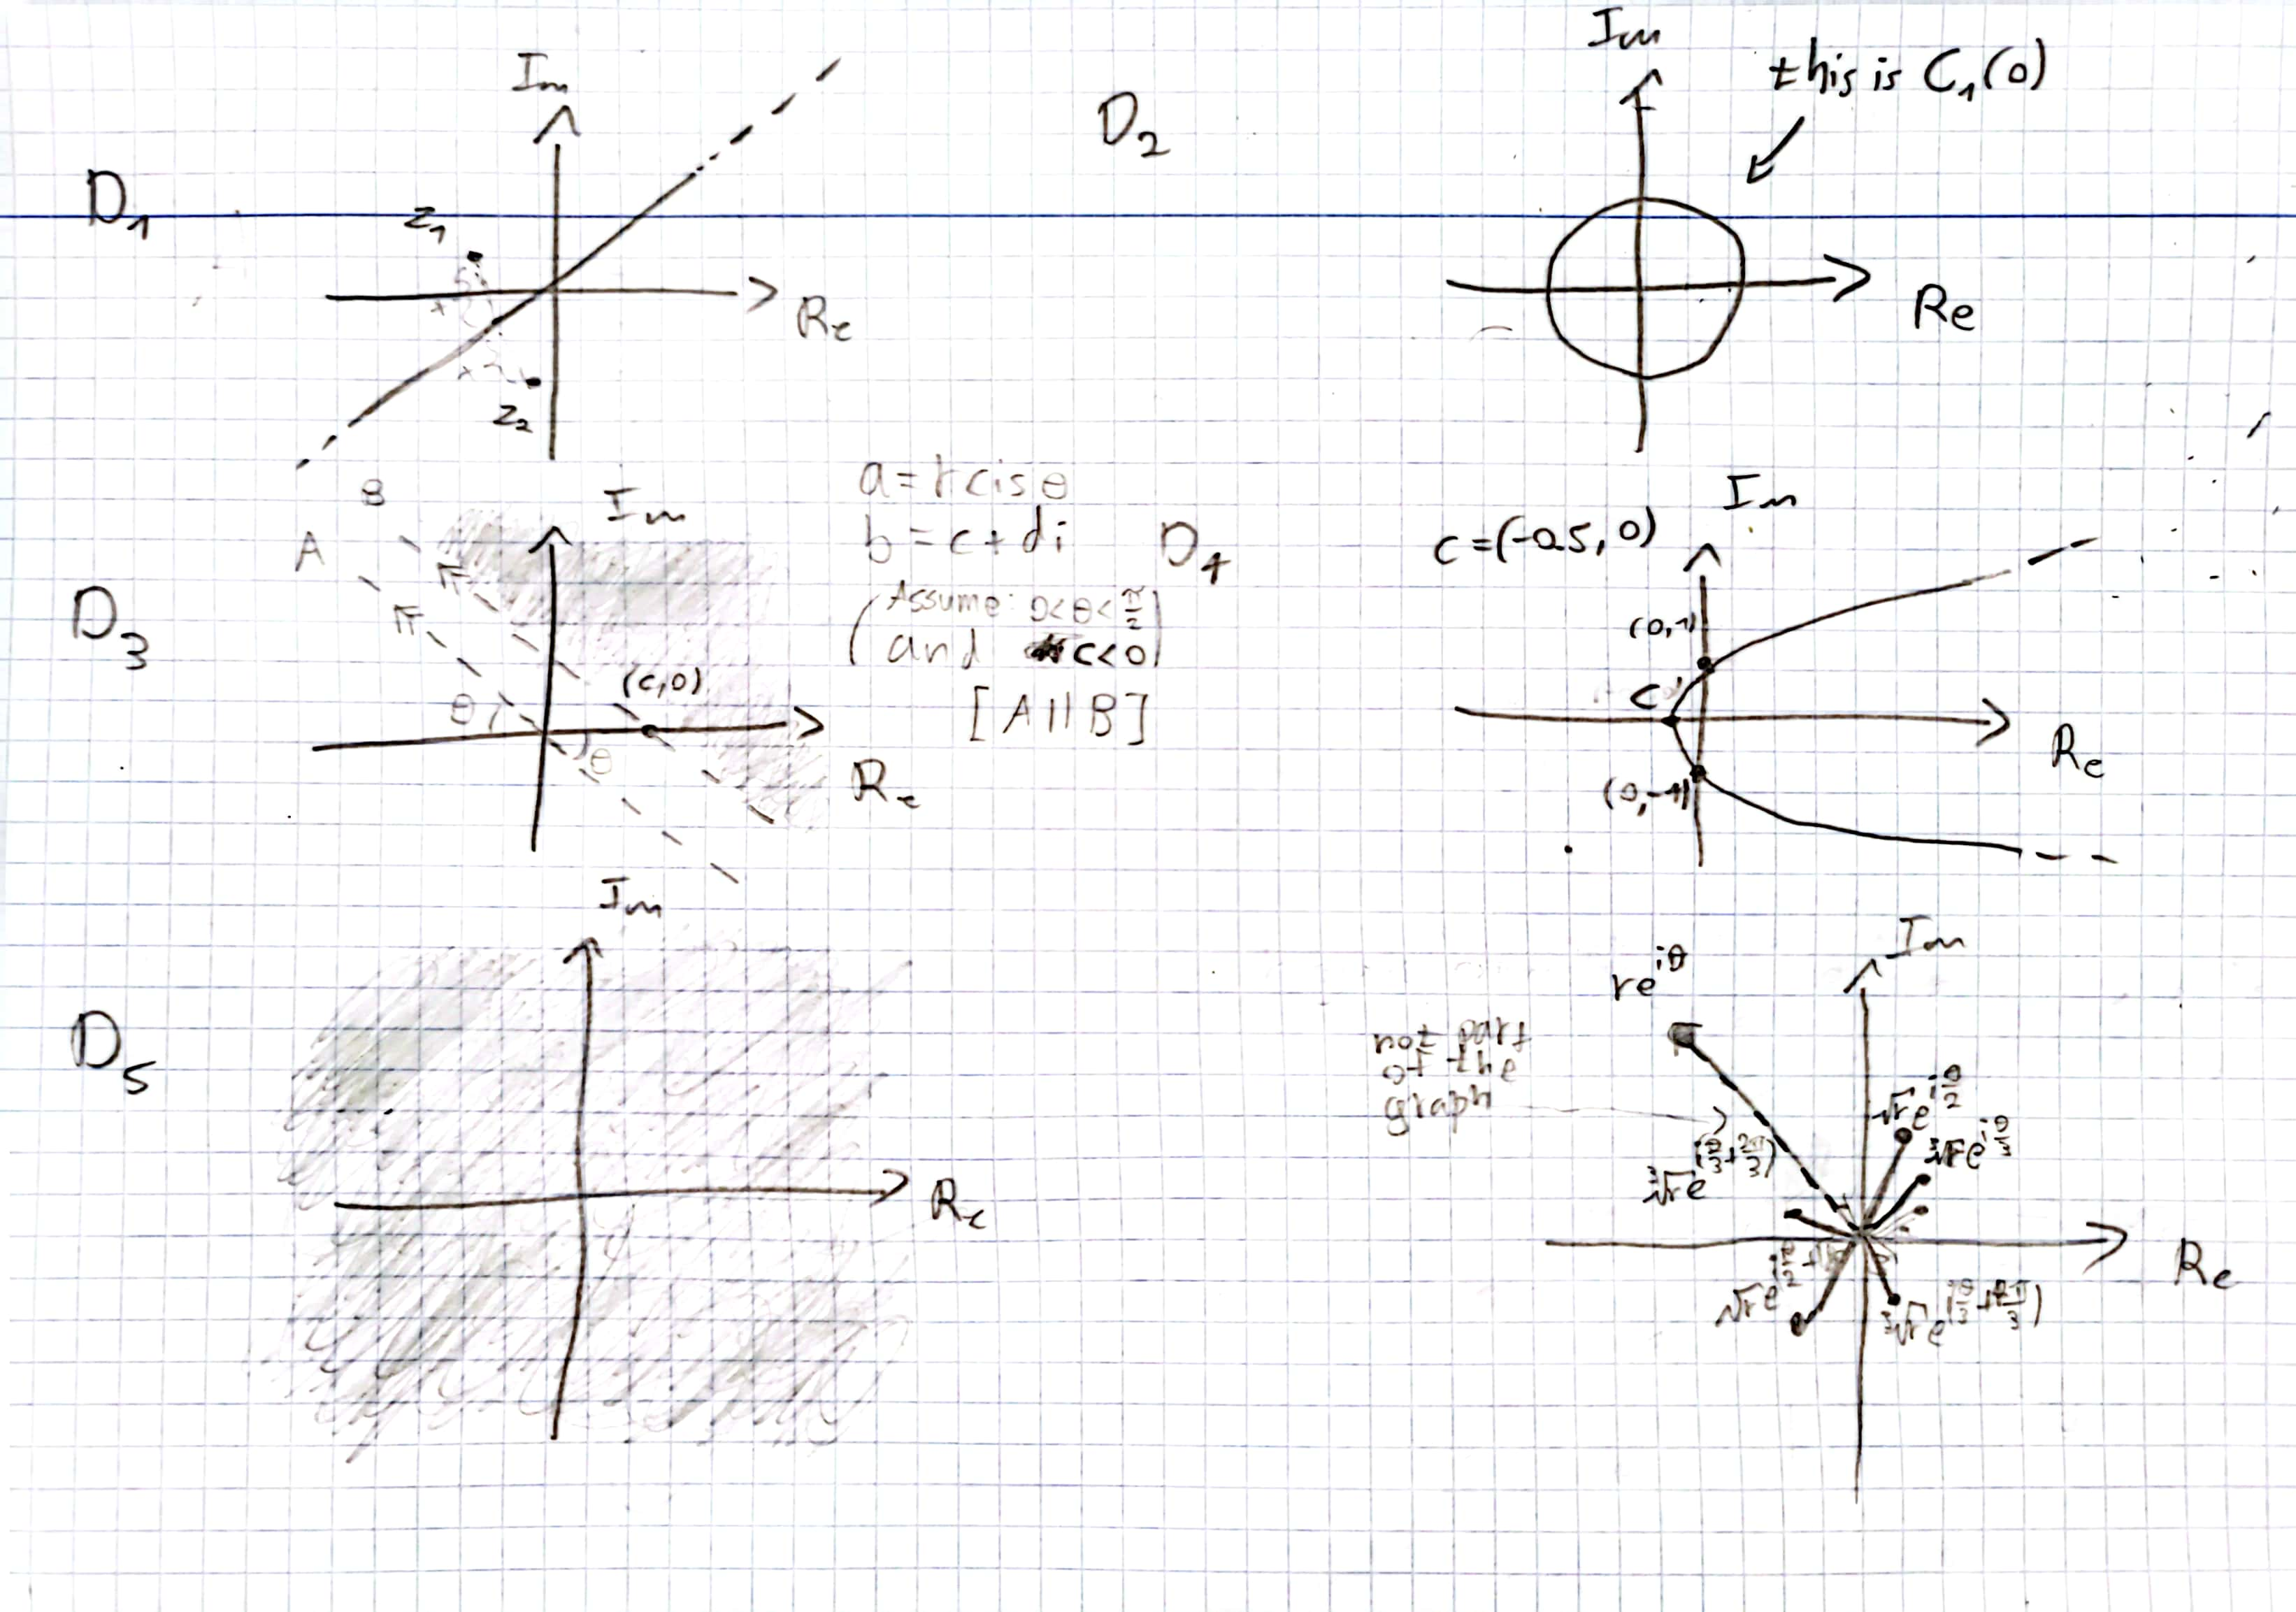
\includegraphics[scale=0.12]{data/complex_analysis/graphes.jpg}
  \end{center}
\end{solution}

\begin{exercise}
  Let $\Omega \subset \C$ be an open connected set.
  Prove that it is path connected.
\end{exercise}
\begin{solution}
  Let $z_0 \in \Omega$ and define the set:
  \[
    U = \set{z \in \Omega \mid 
    \text{there exists a path from $z_0$ to $z$ in $\Omega$}}.
  \]
  We know that $U$ is not empty because $z_0 \in U$.
  Since $\Omega$ is open we know that for any $z \in U \subset \Omega$ exists 
  some $r > 0$ such that $B(z,r) \subset \Omega$.
  Because any point $z' \in B(z,r)$ can be path connect to $z$ by
  the path
  \[
    u(t) = z + (w - z) t, t \in [0,1]
  \]
  we can see that by concatenating the path from $z_0$ to $z$ and $u(t)$
  that $z' \in U$.
  Since this is true for any $z' \in B(z,r)$ we have $B(z,r) \subset U$
  and therefore that $U$ is an open subset of $\Omega$.

  Since $z \in U^c \subset \Omega$ and $\Omega$ is open, there exists $r > 0$
  such that $B(z,r) \subset \Omega$.
  Because of what we saw earlier (an open ball is path connected), it is
  clear that if there exists a path from $z_0$ to some point in $B(z,r)$
  we would get that $z \in U$ which is a contradiction.
  This shows that $U^c$ is open, which means that $U$ is a closed subset of
  $\Omega$.

  We know that $U$ is not empty, and we have just shown it is both open and 
  closed in $\Omega$. 
  This means that $U \cup U^c$ is a union of disjoint open sets that is equal 
  to $\Omega$, and since $U$ is not empty, and $\Omega$ is connected, 
  we must have $U = \Omega$. Since the choice of $z_0$ was arbitrary, 
  for any $z_0 \in \Omega$ the set $U = \Omega$, so $\Omega$ is 
  path connected which completes the proof.
\end{solution}

\newpage

\subsection{Blaschke factor}

\begin{exercise}
  Let $z$, $w$ be complex numbers such that $z \bar w \neq 1$.
  Prove that if $|z| < 1$ and $|w| < 1$, then
  \[
    \abs{\frac{w - z}{1 - \bar w z}} < 1,
  \]
  and if $|w| = 1$ or $|z| = 1$, then
  \[
    \abs{\frac{w - z}{1 - \bar w z}} = 1.
  \]
  We will come back to this result later.
\end{exercise}
\begin{solution}
  We have that
  \[
    \abs{\frac{w - z}{1 - \bar w z}} < 1 \iff
    |w - z| < |1 - \bar w z| \iff
    |w - z|^2 < |1 - \bar w z|^2
  \]
  and since we have
  \begin{align*}
    |w - z|^2 &= (w - z) \overline{(w - z)} = (w - z)(\bar w - \bar z) \\
    |1 - \bar w z|^2 &= (1 - \bar w z)\overline{(1 - \bar w z)} =
    (1 - \bar w z)(1 - w \bar z)
  \end{align*}
  we just need to prove
  \[
    (w - z)(\bar w - \bar z) < (1 - \bar w z)(1 - w \bar z) \iff
    |w|^2 + |z|^2 < 1 + |w|^2 |z|^2
  \]
  which is equivalent to
  \[
    |w|^2 (1 - |z|^2) < 1 - |z|^2
  \]
  and that is true because $|w| < 1$ and $|z| < 1$ which completes the first 
  part of the exercise.

  From the exact calculations above we have that
  \[
    \abs{\frac{w - z}{1 - \bar w z}} = 1 \iff
    |w|^2 + |z|^2 = 1 + |w|^2 |z|^2
  \]
  so if we have $|z| = 1$ or $|w| = 1$ we get the expressions
  \[
    |w|^2 + 1 = 1 + |w|^2
    \tand
    1 + |z|^2 = 1 + |z|^2
  \]
  that are both always true, which completes the second part of the exercise.
\end{solution}

\newpage

\section{Holomorphic functions}
\subsection{Holomorphicity verification}

\begin{exercise}
  Given that
  \begin{itemize}
    \item $\diffp{}{z}(f \pm g) = \diffp{f}{z} \pm \diffp{g}{z}$ and 
      $\diffp{}{{\bar z}}(f \pm g) = \diffp{f}{{\bar z}} \pm \diffp{g}{{\bar z}}$
    \item $\diffp{}{z}(f g) = f\diffp{g}{z} + g\diffp{f}{z}$ and 
      $\diffp{}{{\bar z}}(f g) = f\diffp{g}{{\bar z}} + g\diffp{f}{{\bar z}}$
    \item $\overline{\diffp{f}{z}} = \diffp{{\bar f}}{{\bar z}}$ and
      $\overline{\diffp{f}{{\bar z}}} = \diffp{{\bar f}}{z}$
  \end{itemize}
  Show that the complex chain rules hold
  \[
    \diffp{(g \circ f)}{z} =
    \diffp{g}{z} \diffp{f}{z} + \diffp{g}{{\bar z}} \diffp{\bar f}{z} \tand
    \diffp{(g \circ f)}{{\bar z}} =
    \diffp{g}{z} \diffp{f}{{\bar z}} + 
    \diffp{g}{{\bar z}} \diffp{\bar f}{{\bar z}}.
  \]
\end{exercise}
\begin{solution}
  First we remember that we can represent $(x,y)$ with $(z, \bar z)$ so
  we have
  \[
    g \circ f = g(f(z,\bar z),\bar f(z,\bar z)).
  \]
  Using the chain rule from $\R^2$ with $w = f(z, \bar z)$ we now get
  \begin{align*}
    \frac{\partial (g\circ f)}{\partial z} &=
    \frac{\partial (g(f(z,\bar z),\bar f(z,\bar z))}{\partial z} =
    \frac{\partial g(w,\bar w)}{\partial w}
    \frac{\partial f(z,\bar z)}{\partial z} +
    \frac{\partial g(w,\bar w)}{\partial \bar w}
    \frac{\partial \bar f(z,\bar z)}{\partial z} \\ &=
    \del{\diffp{g}{z} \diffp{f}{z} + \diffp{g}{{\bar z}} \diffp{\bar f}{z}}
    (f \circ g)
  \end{align*}
  Given the first chain rule, we can now use it to prove the second one:
  \[
    \overline{\diffp{(g \circ f)}{{\bar z}}} =
    \diffp{(\bar g \circ f)}{z} =
    \diffp{\bar g}{z} \diffp{f}{z} + 
    \diffp{{\bar g}}{{\bar z}} \diffp{\bar f}{z}
  \]
  and from this follows
  \[
    \diffp{(g \circ f)}{{\bar z}} =
    \overline{\diffp{\bar g}{z} \diffp{f}{z} + 
    \diffp{{\bar g}}{{\bar z}} \diffp{\bar f}{z}} =
    \diffp{g}{z} \diffp{f}{{\bar z}} + 
    \diffp{g}{{\bar z}} \diffp{\bar f}{{\bar z}}.
  \]
  Notice that we used the fact addition is commutative in the last equality.
\end{solution}

\begin{exercise}
  Find all the points in the complex plane where the following functions
  are holomorphic:
  \begin{enumerate}
    \item[(1)] $f(z) = e^{z \bar z^2 - 2 \bar z}$.
    \item[(2)] $f(x + i y) = \overline{\sin(\bar z)}$ where
      $\sin(z) := \frac{e^{i z} - e^{-i z}}{2 i}$.
  \end{enumerate}
\end{exercise}
\begin{solution}
  Our strategy for this problem is to use the proposition from the recitations
  that $f$ is holomorphic at $p$ if and only if $\partial_{\bar z} f = 0$.
\begin{enumerate}
\item[(1)] Using the chain rule we have
  \[
    \diffp{f}{{\bar z}} = 
    e^{z \bar z^2 - 2 \bar z}(2 z \bar z - 2) =
    2 e^{z \bar z^2 - 2 \bar z}(|z|^2 - 1) =
    0.
  \]
  This is only true when $|z|^2 = 1$.
  In other words, the function $f(x)$ is holomorphic only on $C_1(0)$.
\item[(2)] Using the conjugation rule we see
  \[
    \diffp{f}{{\bar z}} =
    \overline{\diffp{\sin(\bar z)}{z}} =
    \overline{\diffp{}{z} \frac{e^{i \bar z} - e^{-i \bar z}}{2 i}} = 0
  \]
  so this function is entire.
\end{enumerate}
\end{solution}

\subsection{The Cauchy--Riemann equations}
\begin{exercise}
  Let $\Omega \subset \C$ be a domain (connected and open), let
  $f \colon \Omega \to \C$ be holomorphic, and let $R > 0$.
  Prove or disprove the following:
  \begin{itemize}
  \item[(1)] Let $g(z) := \bar f(\bar z)$ be holomorphic in 
    $\Omega := \set{z \in \C \mid \bar z \in \Omega}$, then $f$ is constant.
  \item[(2)] Let $g(z) := \bar f(z)$ be holomorphic, then $g$ is constant.
  \item[(3)] Suppose $|f(z)| > R$ for all $z \in \Omega$, then $f$ is
    constant.
  \item[(4)] Suppose $|f(z)| = R$ for all $z \in \Omega$, then $f$ is
    constant.
  \end{itemize}
\end{exercise}
\begin{solution} \phantom{}
\begin{enumerate}
\item[(1)] A counter example to this proposition if the function $f(z) = z$.
  We can see that $g(z) = \bar f(\bar z) = \bar {\bar z} = z$ is entire.
  We have that $f$ is holomorphic for example on $\Omega = \C$ but
  $g(z) = z$ is not constant.
\item[(2)] This is true.
  First denote the functions using $f = u + i v$ notation.
  \begin{align*}
    f(x) &= u(x,y) + v(x,y) \\
    g(x) &= \bar f (z) = u(x,y) - v(x,y)
  \end{align*}
  Since both of these functions are entire,
  we can now solve this by using the Cauchy--Riemann equations they satisfy:
  \begin{gather}
    \diffp{u}{x} = \diffp{v}{y} \stand \diffp{u}{y} = - \diffp{v}{x} \\
    \diffp{u}{x} = - \diffp{v}{y} \stand \diffp{u}{y} = \diffp{v}{x}
  \end{gather}
  After summing equations $(1)$ and $(2)$, we get that
  \[
    \diffp{u}{x} = \diffp{u}{y} = 0,
  \]
  and putting this back into the equation we also get that
  \[
    \diffp{v}{x} = \diffp{v}{y} = 0,
  \]
  which implies that $f$ is constant, and completes the proof.
\item[(3)] A counter example for this proposition is 
  the function $f(z) = z$ on $\Omega = \C \setminus D_1(0)$.
  It is obvious that for any $z \in \Omega$ that 
  \[
    |f(z)| = |z| > D.
  \]
  However, the function is clearly not constant.
  \setcounter{equation}{0}
\item[(4)] This is true.
  We can prove this by first write the result of the function in polar form:
  \[
    f(z) = R \cis(u(x,y)) = R \sin(u(x,y)) + i R \cos(u(x,y))
  \]
  for a real valued function $u(x,y)$.
  This gives the Cauchy--Riemann equations:
  \begin{gather}
    R \cos(u(x,y)) \diffp{u}{x} = - R \sin(u(x,y)) \diffp{u}{y} \\
    R \cos(u(x,y)) \diffp{u}{y} = R \sin(u(x,y)) \diffp{u}{x}
  \end{gather}
  Dividing equations $(1)$ and $(2)$ by $R \neq 0$ we get:
  \begin{gather}
    \cos(u(x,y)) \diffp{u}{x} = - \sin(u(x,y)) \diffp{u}{y} \\
    \cos(u(x,y)) \diffp{u}{y} = \sin(u(x,y)) \diffp{u}{x}
  \end{gather}
  For any given point, we have that either $\cos(u(x,y))$ or $\sin(u(x,y))$
  are different than $0$. Without loss of generality assume that
  $\cos(u(x,y)) \neq 0$.
  We can now divide by $\cos(u(x,y))$ and combine equations $(4)$ and $(5)$
  to get
  \[
    \cos(u(x,y)) \diffp{u}{y} =
    \sin(u(x,y)) \del{- \tan(u(x,y)) \diffp{u}{y}}
  \]
  which implies that
  \[
    \diffp{u}{y} =
    \underbrace{- \tan^2(u(x,y))}_{\neq\,1} \diffp{u}{y} \implies
    \diffp{u}{y} = 0.
  \]
  From equation $(3)$ and $\cos(u(x,y)) \neq 0$ it is clear that this
  implies that $\diffp{u}{x} = 0$ which implies that $u(x,y)$ and thus $f$
  is constant.
\setcounter{equation}{0}
\end{enumerate}
\end{solution}

\subsection{Harmonic functions}
Let $\Omega \subset \C$ and 
$U := \set{(x,y) \in \R^2 \mid x + i y \in \Omega}$.
\begin{exercise}
  We know from the recitations that if $f = u + i v$ is differentiable twice,
  then $u$, $v$ are both harmonic functions.
  In this exercise, we will show the opposite direction of this proposition
  locally.
  Suppose that $u(x,y)$ has continuous partial derivatives up to $2$nd order
  and is harmonic ($\Delta f = 0$) in $U$.
  Show that for any $(x_0, y_0) \in U$ the function
  \[
    v(x,y) =
    \int_{y_0}^{y} \diffp{u}{x}(x,s) \ds -
    \int_{x_0}^{x} \diffp{u}{y}(t,y_0) \dt
  \]
  is harmonic, and also satisfies the Cauchy--Riemann equations with $u$.
  Conclude that $f = u + i v$ defined by these functions is a holomorphic
  function.
\end{exercise}
\begin{solution}
  Let us compute the partial derivatives of the function:
  \begin{align*}
    \diffp{}{x} v(x,y) &= \diffp{}{x} \int_{y_0}^{y} \diffp{u}{x}(x,s) \ds -
    \int_{x_0}^{x} \diffp{u}{y}(t,y_0) \dt
                       &= \diffp{}{x} \int_{y_0}^{y} \diffp{u}{x}(x,s) \ds -
                          \diffp{}{x} \int_{x_0}^{x} \diffp{u}{y}(t,y_0) \dt
  \end{align*}
  We have that
  \begin{align*}
    \diffp{}{x} \int_{y_0}^{y} \diffp{u}{x}(x,s) \ds &=
    \int_{y_0}^{y} \diffp[2]{u}{x}(x,s) \ds \underset{u \text{ harmonic}}{=}
    - \int_{y_0}^{y} \diffp[2]{u}{y}(x,s) \ds =
    \diffp{u}{x}(x,y_0) - \diffp{u}{x}(x,y) \\
    \diffp{}{x} \int_{x_0}^{x} \diffp{u}{y}(t,y_0) \dt &=
    \diffp{u}{y}(x,y_0)
  \end{align*}
  so it follows that
  \begin{equation}
    \label{eq:cro}
    \diffp{v}{x}(x,y) =
    \diffp{u}{x}(x,y_0) - \diffp{u}{x}(x,y) - \diffp{u}{x}(x,y_0) =
    - \diffp{u}{x}(x,y).
  \end{equation}
  On the other hand, we have that
  \begin{align*}
    \diffp{}{y} v(x,y) &= \diffp{}{y} \int_{y_0}^{y} \diffp{u}{x}(x,s) \ds -
    \int_{x_0}^{x} \diffp{u}{y}(t,y_0) \dt
                       &= \diffp{}{y} \int_{y_0}^{y} \diffp{u}{x}(x,s) \ds -
                          \diffp{}{y} \int_{x_0}^{x} \diffp{u}{y}(t,y_0) \dt
  \end{align*}
  and
  \begin{align*}
    \diffp{}{y} \int_{y_0}^{y} \diffp{u}{x}(x,s) \ds &=
    \diffp{u}{x}(x,y) \\
    \diffp{}{y} \int_{x_0}^{x} \diffp{u}{y}(t,y_0) \dt &=
    0
  \end{align*}
  which implies that
  \begin{equation}
    \label{eq:crt}
    \diffp{v}{y}(x,y) = \diffp{u}{x}(x,y).
  \end{equation}
  We notice that \cref{eq:cro,eq:crt} are the Cauchy--Riemann equations,
  which is just what we wanted to prove.
  To show that $v(x,y)$ is a harmonic function we can use
  \cref{eq:cro,eq:crt} again to obtain
  \begin{gather}
    \diffp{v}{x} = - \diffp{u}{y} \implies \diffp[2]{v}{x} = - \diffp{u}{xy} \\
    \diffp{v}{y} = \diffp{u}{x} \implies 
    \diffp[2]{v}{y} = \diffp{u}{yx}
  \end{gather}
  but since $u \in C(\R^2)$ from Schwarz's theorem we have
  \[
    \diffp{u}{xy} = \diffp{u}{yx}
  \]
  which in turn implies that
  \[
    \diffp[2]{v}{x} + \diffp[2]{v}{y} = 0
  \]
  so $v$ is a harmonic function as wanted which completes the proof.
\end{solution}

\begin{exercise}
  Let $u$, $v$ be conjugate harmonic in $U$.
  Show that
  \[
    \varphi(x,y) = - \frac{v(x,y)}{u^2(x,y) + v^2(x,y)}
  \]
  is harmonic in $U$.
  Recall the formula $\Im(\frac{1}{z}) = - \frac{y}{x^2 + y^2}$.
\end{exercise}
\begin{solution}
  First denote
  \[
    f(z) := u(x,y) + i v(x,y)
  \]
  which is a holomorphic function.
  From the hint we obtain that
  \[
    \Im\del{\frac{1}{f(z)}} = \frac{v(x,y)}{u^2(x,y) + v^2(x,y)}.
  \]
  We know that the if $f$ is holomorphic that $1/f$ is also holomorphic,
  and as a result of the recitations we have that $\Im(1/f)$ is also
  holomorphic.
\end{solution}

\begin{exercise}
  For $u = e^{x^2 - y^2} \cos(2 x y)$, find a harmonic function
  $v$ such that $f = u + i v$ is entire.
\end{exercise}
\begin{solution}
  We can find the appropriate function $v(x,y)$ as it's defined in
  the previous exercises.
  \begin{align*}
    \diffp{u}{x} &= 2 x e^{x^2 - y^2} \cos(2xy) - 2 y \sin(2xy) e^{x^2 - y^2} \\
    \diffp{u}{y} &=
    - 2 y e^{x^2 - y^2} \cos(2xy) - 2 x \sin(2xy) e^{x^2 - y^2}
  \end{align*}
  We can choose aribirarily choose $x_0 = y_0 = 0$ and then
  \[
    v(x,y) =
    \int_{0}^{y} \diffp{u}{x}(x,s) \ds -
    \int_{0}^{x} \diffp{u}{y}(t,0) \dt =
  \]
  and calculating the integrals we get:
  \begin{align*}
    \int_{0}^{y} \diffp{u}{x}(x,s) \ds &=
    \int_{0}^{y} 2 x e^{x^2 - s^2} \cos(2xs) - 2 s \sin(2xs) e^{x^2 - s^2} \ds
    \\ &= e^{x^2 - s^2} \cos(2 x s) \vert^y_0 \\ &= e^{x^2 - y^2} \sin(2 x y)
  \end{align*}
  where the last calculation follows from linearity and integration by parts,
  and
  \begin{align*}
    \int_{0}^{x} \diffp{u}{y}(t,0) \dt &=
    \int_{0}^{x} 
    - 2 \times 0 \times  e^{t^2} \cos(2t) - 2 t \sin(0) e^{t^2} \dt = 0,
  \end{align*}
  so finally we have
  \[
    v(x,y) = e^{x^2 - y^2} \sin(2 x y)
  \]
  which implies $f$ is holomorphic where $u$ is harmonic, so since $u$ is
  a harmonic function on $\C$, we get $f$ is entire.
\end{solution}

\newpage

\section{Analytic functions}
\subsection{Convergence radius}

\begin{exercise}
  Prove the following:
  \begin{enumerate}
    \item[(a)] The power series $\sum n z^n$
      does not converge on any point of the unit circle.
    \item[(b)] The power series $\sum z^n/n^2$
      converges at every point of the unit circle.
    \item[(c)] The power series $\sum z^n/n$
      converges at every point of the unit circle except $z = 1$.
  \end{enumerate}
\end{exercise}
\begin{solution} \phantom{}
  \begin{enumerate}
    \item[(a)] Let $z \in C_1(0)$.
      Assume, by way of contradiction,
      that the series is bounded by $M > 0$.
      Denote the series of partial sums $S_n$.
      Since the series is bounded by $M$ we have $S_{2M} \in D_{M}(0)$.
      However, we have
      \[
        S_{2M + 1} = S_{2M} + (2M + 1) z^{2M + 1},
      \]
      which implies that
      \[
        \abs{S_{2M + 1} - S_{2M}} = 2M + 1 > 2M.
      \]
      Therefore from $\diam(D_{M}(0)) = 2M$
      we obstain $S_{2M + 1} \notin D_{M}(0)$.
      This contradiction implies that the series is not bounded for any
      $z \in C_1(0)$ and in particular it does not converge on the unit circle.
    \item[(b)] Let $z \in C_1(0)$.
      We can write $z = e^{i \theta}$ for some $\theta \in [0,2\pi)$ so
      \[
        \sum_{n=1}^{\infty} \frac{z^n}{n^2} =
        \sum_{n=1}^{\infty} \frac{e^{i \theta n}}{n^2}.
      \]
      We know that the series $\sum_{n=1}^{\infty} \frac{1}{n^2}$ converges.
      Therefore, since
      \[
        \abs{\frac{e^{i \theta n}}{n^2}} \le \frac{1}{n^2},
      \]
      by the comparison test, the series converges for any $z \in C_1(0)$.
    \item[(c)] When $z = 1$ we get the harmonic series which we know diverges.
      Fix $1 \neq z \in C_1(0)$.
      We want to apply Dirichlet's test.
      The partial sums form a geometric sum
      \[
        A_n =
        \sum_{k=1}^{n} e^{i \theta k} =
        e^{i \theta} \frac{1 - e^{i \theta n}}{1 - e^{i \theta}}.
      \]
      We therefore have
      \[
        |A_n| =
        \abs{\frac{1 - e^{i \theta n}}{1 - e^{i \theta}}} \le
        \frac{2}{\abs{1 - e^{i \theta}}}
      \]
      which means that the partial sums $A_n$ are bounded.
      The sequence $b_n = 1/n$ is clearly decreasing and clearly
      $b_n \to 0$ which means that $\sum z^n / n$ converges on the unit
      circle except at $z = 1$.
  \end{enumerate}
\end{solution}

\begin{exercise}
  \label{ex:convergence-radius-2}
  Let $k \in \N$.
  What is the domain of convergence of the series
  $\sum_{n=1}^{\infty} \frac{z^{nk}}{n}$?
\end{exercise}
\begin{solution}
  For the series $\sum_{n=1}^{\infty} \frac{z^{nk}}{n}$,
  we take
  \[
    a_n =
    \begin{cases}
      \frac{1}{n k^{-1}}, &n k^{-1} \in \N \\
      0, &\text{otherwise}
    \end{cases}
  \]
  so its radius of convergence is
  \[
    \limsup_{n \to \infty} \abs{\frac{1}{n k^{-1}}}^{\frac{1}{n}} = 1.
  \]
  So the series converges when $|z| < 1$ and diverges when $|z| > 1$.
  When $|z| = 1$ we may denote $z = e^{i \theta}$ for $\theta \in [0,2\pi)$.
  We then get
  \[
    \sum_{n=1}^{\infty} \frac{z^{nk}}{n} =
    \sum_{n=1}^{\infty} \frac{e^{i \theta nk}}{n}.
  \]
  It is clear that the series diverges when $e^{i \theta k} = 1$ because
  then the series is the harmonic series.
  When $e^{i \theta k} \neq 1$, we can denote $a_n = 1 / n$
  and $b_n = e^{i \theta n k}$.
  We see that $a_n \to 0$ as $n \to \infty$ and also that
  \[
    B_N =
    \sum_{n=1}^{N} b^n =
    \sum_{n=1}^{N} e^{i \theta nk}.
  \]
  We can denote $z_0 = e^{i \theta k}$ and notice that this is a geometric
  series so
  \[
    \abs{B_N} =
    \abs{\sum_{n=1}^{N} z_0^{k}} =
    \abs{\frac{z_0 \del{1 - z_0^N}}{1 - z_0}} =
  \frac{\abs{1 - z_0^N}}{{\abs{1 - z_0}}} \le K
  \]
  for some $K > 0$ for all $N \in \N$
  where the last step inequality follows from the fact $\abs{1 - z_0}$
  is constant and $\abs{1 - z_0^N}$ is bounded by $2$ since $|z_0| = 1$.
  Using the results above we can conclude that for $e^{i \theta k} \neq 1$
  the series converges by Dirichlet's test.
\end{solution}

\subsection{Product and composition of power series}
\label{ssec:products-compositions-of-power-series}
\begin{exercise}
  Let $g$, $h$ be analytic at around $z_0$.
  Prove that $g \cdot h$ is analytic around $z_0$.
  Conclude that for all $n \in \N$ the function $g^n$ is analytic around $z_0$.
\end{exercise}
\begin{solution}
  Without loss of generality assume $z_0 = 0$.
  Let
  \begin{align*}
    &g(z) := \sum_{k=0}^{\infty} a_k z^k \\
    &h(z) := \sum_{k=0}^{\infty} b_k z^k
  \end{align*}
  Also set
  \[
    A_n := \sum_{k=0}^n a_k x^k \tand
    B_n := \sum_{k=0}^n b_k x^k \tand
    c_r := \sum_{k=0}^r a_{r-k}b_k \tand
    C_n:=\sum_{r=0}^n c_r x^r.
  \]
  Let $\rho$ be the minimal radius of convergence of the power series,
  and let $|x| < \rho$ be given.
  For any $N \geq 1$ the expression $A_N B_N - C_N$ only contains terms
  of the form $a_j b_k x^{j + k}$ where at least one of $j$, $k$ is
  greater than $N / 2$.
  It follows that
  \[
    |A_N B_N - C_N| \le
    \sum_{j>N/2} |a_j x^j| \sum_{k=0}^\infty |b_k x^k| +
    \sum_{j=0}^\infty |a_jx^j| \sum_{k>N/2} |b_k x^k|.
  \]
  Since $g$, $h$ are analytic, the infinte sums both converge and are thus
  bounded, and the finite sums both converge to $0$ as $N \to \infty$
  which means that the entire expression converges to $0$ as $N \to \infty$
  and thus,
  \[
    \lim_{N \to \infty} C_N =
    \lim_{N \to \infty} A_N
    \lim_{N \to \infty} B_N =
    \sum_{j=0}^\infty a_j x^j \cdot \sum_{k=0}^\infty b_k x^k.
  \]
  This shows that $g \cdot h$ is analytic around $z_0$,
  the corollary that $g^n$ is analytic is an immediate result, since
  it is just a special case of the result.
\end{solution}

\begin{exercise}
  \label{ex:composition-of-analytic-is-analytic}
  Let $f$ be analytic around $w_0$ and let $g$ be analytic around $z_0$ such
  that $g(z_0) = w_0$.
  Prove that $f \circ g$ is analytic around $z_0$.
  You may find the following proposition helpful.
  \begin{proposition}
    Let $\set{a_{j,k}}_{j,k \in \N}$ be a sequence such that
    \[
      \sum_{j=1}^{\infty} \del{\sum_{k=1}^{\infty} \abs{a_{j,k}}} < \infty.
    \]
    Then
    \[
      \sum_{k=1}^{\infty} \sum_{j=1}^{\infty} a_{j,k} = 
      \sum_{j=1}^{\infty} \sum_{k=1}^{\infty} a_{j,k}.
    \]
  \end{proposition}
\end{exercise}
\begin{solution}

\end{solution}

\begin{exercise}
  Prove that $f(z) = e^{\frac{2 \pi}{z}}$ is analytic on $\C \setminus \set{0}$.
\end{exercise}
\begin{solution}
  We have seen in class that $e^z$ is entire,
  and we know that $2\pi \frac{1}{z}$ is analytic on $\C \setminus \set{0}$.
  Using the result from \Cref{ex:composition-of-analytic-is-analytic}
  the proof for this exercise is complete.
\end{solution}

\subsection{Power series and the uniqueness theorem}
\begin{exercise}
  \label{ex:power-series-calc}
  Find the power series expansion of $f(z) = \frac{z}{z^2 + 1}$ around the
  origin.
  What is the disc of convergence of that series?
\end{exercise}
\begin{solution}
  We can rewrite the function as
  \[
    f(z) = z \cdot \frac{1}{1 + z^2}.
  \]
  Then by using results from \Cref{ssec:products-compositions-of-power-series}
  we can conclude that the power series for this function is
  \[
    f(z) =
    z \sum_{n=0}^{\infty} (-1)^n z^{2n} =
    \sum_{n=0}^{\infty} (-1)^n z^{2n + 1}.
  \]
  We can calculate the disc of convergence by the Cauchy--Hadamard theorem
  of by noticing the radii of the power series of the functions we composed.
  The radius is given by
  \[
    R = \frac{1}{\limsup\limits_{n \to \infty} |a_n|^{\frac{1}{n}}} = 1.
  \]
\end{solution}

\begin{exercise}
  \label{ex:find-all-function-st}
  Find all the analytic functions $f \colon D_1(0) \to \C$ such that
  \[
    f\del{\frac{i}{n}} = \frac{n i}{n^2 - 1}
  \]
  for all $n > 1$.
\end{exercise}
\begin{solution}
  Write
  \[
    f(z) = \sum_{k=0}^{\infty} a_k z^k.
  \]
  Subtituting the given points we have
  \[
    f\del{\frac{i}{n}} =
    \sum_{k=0}^{\infty} a_k \del{\frac{i}{n}}^k =
    \frac{n i}{n^2 - 1} =
    \frac{\frac{i}{n}}{1 - \frac{1}{n^2}} =
    \frac{i}{n} \sum_{k=0}^{\infty} \del{\frac{1}{n^2}}^k =
    \sum_{k=0}^{\infty} \frac{i}{n^{2k+1}}.
  \]
  This means that
  \[
    \sum_{k=0}^{\infty} a_k \del{\frac{i}{n}}^k =
    \sum_{k=0}^{\infty} \frac{i}{n^{2k+1}}
  \]
  so the even coefficients must be zero,
  and the odd coefficients must be $a_{2k+1} = (-1)^k$.
  It follows that the power series is
  \[
    f(z) =
    \sum_{n=0}^{\infty} (-1)^n z^{2n + 1}.
  \]
  This is exactly the power series from \Cref{ex:power-series-calc}!
  From the uniqueness theorem it follows that our function must be
  \[
    f(z) = \frac{z}{z^2 + 1}.
  \]
\end{solution}

\begin{exercise}
  Find at least two analytic functions
  $f_1,f_2 \colon D_1(0) \setminus {0} \to \C$ such that
  \[
    f\del{\frac{i}{n}} = \frac{n i}{n^2 - 1}
  \]
  for all $n > 1$.
  What is the difference from the previous exercise in this case?
\end{exercise}
\begin{solution}
  Using the result from \Cref{ex:find-all-function-st}
  we immediately get the function
  \[
    f_1(z) = \frac{z}{z^2 + 1}.
  \]
  We can also define
  \[
    f_2(z) = \frac{z}{z^2 + 1} + \sin\del{\frac{\pi}{i z}}.
  \]
  It is we defined on the punctured disc $D_1(0) \setminus \set{0}$ and
  it clearly vanishes at $z_k = \frac{i}{k}$ for $k > 1$ since
  \[
    \sin\del{\frac{\pi}{i z_k}} =
    \sin\del{- k \pi} = 0.
  \]
  This completes the proof.
\end{solution}

\newpage

\section{Primitive functions and the complex integral}
\subsection{Convex regions}
\begin{exercise}
  Let $\Omega \subset \C$ be a convex region
  and let $f = u + i v \colon \Omega \to \C$
  be a holomorphic function such that $f'(z)$ is continuous.
  Set $z_0 \in \Omega$ and define
  \[
    F(z) := \int\limits_{[z_0,z]} f(w) \dw.
  \]
  Write the integral explicitly by choosing the right path, and prove
  that $F(z)$ is the antiderivative of $f$ in $\Omega$.
\end{exercise}
\begin{solution}
  First define the function $g(z) := f(z + z_0)$, and the following paths
  \begin{align*}
    \gamma_1(t) &= z_0 + t(z - z_0), \quad t \in [0,1] \\
    \gamma_1'(t) &= z - z_0 \\
    \gamma_2(t) &= t(z - z_0), \quad t \in [0,1] \\
    \gamma_2'(t) &= z - z_0
  \end{align*}
  Since $\Omega$ is convex, the function $f$ is defined on all of them we
  we get that
  \begin{align*}
    \int\limits_{[z_0,z]} f(w) \dw &=
    \int_{0}^{1} f(\gamma_1(t)) \cdot \gamma_1'(t) \dt =
    \int_{0}^{1} f(z_0 + t(z - z_0)) \cdot (z - z_0) \dt \\ &=
    \int_{0}^{1} g(t(z - z_0)) \cdot (z - z_0) \dt =
    \int_{0}^{1} g(\gamma_2(t)) \cdot \gamma_2'(t) \dt =
    \int\limits_{[0,z-z_0]} f(w) \dw.
  \end{align*}
  Thus we could assume without loss of generaility that $z_0 = 0$.
  For $h > 0$ such that $B(z,h) \subset \Omega$ we have that
  \begin{align*}
    \frac{F(z + h) - F(z)}{h} &=
    \frac{1}{h} \del{\int_{0}^{1} f(t(z + h)) \cdot
    (z + h) \dt - \int_{0}^{1} f(tz) \cdot z \dt} \\ &=
    \int_{0}^{1} \frac{f(t(z + h)) \cdot (z + h) - f(tz) \cdot z}{h} \dt.
  \end{align*}
  Since the functions $z$, $tz$, $f(z)$ are holomorphic, and since
  the composition and product of holomorphic functions is holomorphic we
  get that
  \[
    \frac{f(t(z + h)) \cdot (z + h) - f(tz) \cdot z}{h}
    \taking{h \to 0} \diff{{(f(tz) \cdot z)}}{z}.
  \]
  Since the product of continuosly differentiable functions is continuously
  differentiable, we get that
  \begin{align*}
    \lim_{h \to 0}
    \int_{0}^{1} \frac{f(t(z + h)) \cdot (z + h) - f(tz) \cdot z}{h} &=
    \int_{0}^{1} 
    \lim_{h \to 0} \frac{f(t(z + h)) \cdot (z + h) - f(tz) \cdot z}{h} \\ &=
    \lim_{h \to 0} \diff{{(f(tz) \cdot z)}}{z} =
    \lim_{h \to 0}  \frac{F(z + h) - F(z)}{h} = F'(z).
  \end{align*}
  This means that $F'(z)$ exists and thus $F$ is holomorphic.
  We also see that
  \begin{align*}
    F'(z) &= \int_{0}^{1} \diff{{(f(tz) \cdot z)}}{z} \dt \\
          &= \int_{0}^{1} [f'(tz) \cdot tz + f(tz)] \dt \\
          &= \int_{0}^{1} \diff{{(t \cdot f(tz))}}{t} \dt
          = [t \cdot f(z)] \vert_{t=0}^{t=1} = f(z).
  \end{align*}
  This shows that $F$ is the antiderivative of $f$ on $\Omega$ which completes
  the proof.
\end{solution}

\subsection{Improper real integrals}

\begin{exercise}
  Let $w < 0$ be given.
  \begin{enumerate}
    \item[(1)] For $\epsilon > 0$ denote $Q_{\epsilon}$ the positivly oriented
      square path with edges of length $\epsilon$ around $i$.
      Denote $\gamma_R$ the half circle path around the origin (with radius
      $R$) united with the interval $[-R,R]$ such that it is positively
      oriented.
      For a sufficiently small $\epsilon > 0$, prove that
      \[
        \int_{\gamma_R} \frac{e^{i w z}}{1 + z^2} \dz =
        \int_{Q_{\epsilon}} \frac{e^{i w z}}{1 + z^2} \dz.
      \]
      You may assume that $R > 1$.
    \item[(2)] Calculate the limits
      \[
        \lim_{R \to \infty} \int_{\gamma_R} \frac{e^{i w z}}{1 + z^2} \dz
        \tand
        \lim_{\epsilon \to 0^+}
        \int_{Q_{\epsilon}(i)} \frac{e^{i w z}}{1 + z^2} \dz
      \]
    \item[(3)] Calculate
      \[
        \int_{\ninfty}^{\infty} \frac{e^{i w t}}{1 + t^2} \dt.
      \]
  \end{enumerate}
  \begin{figure}[H]
  \centering
  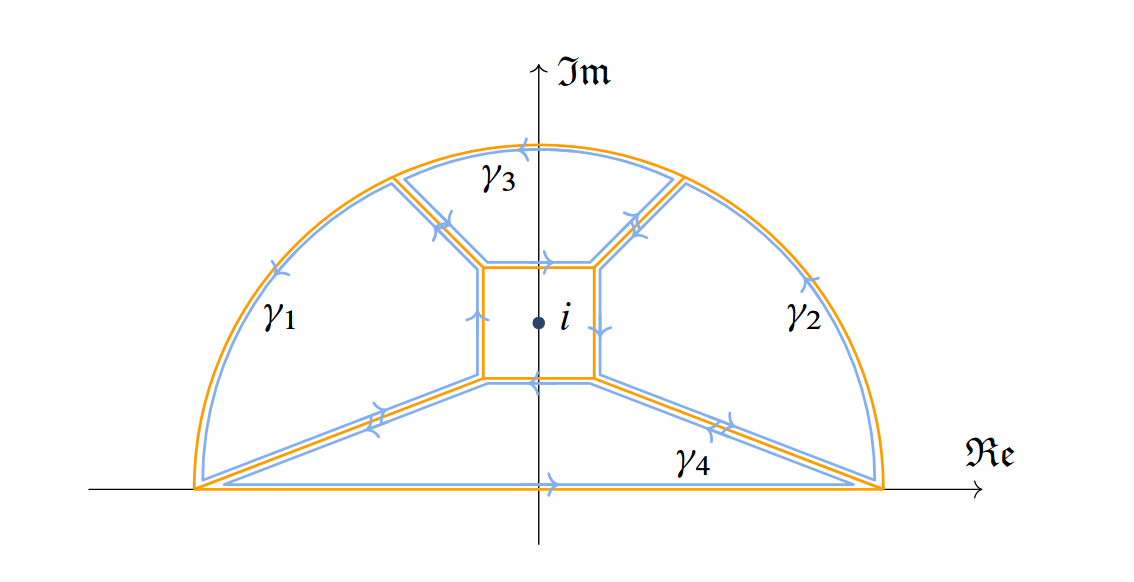
\includegraphics[scale=0.25]{data/complex_analysis/hw4q2.png}
  \end{figure}
\end{exercise}
\begin{solution} \phantom{}
\begin{enumerate}
  \item[(1)] Since $R > 1$ there exists $\epsilon > 0$ such that
    \[
      \abs{\frac{\epsilon}{2} + i \del{\frac{\epsilon}{2} + 1}} < R
    \]
    and thus the square path will be properly contained in the half circle
    of radius $R$.
    We can see that
    \[
      \sum_{j=1}^{4} \int_{\gamma_{j}} \frac{e^{-i w z}}{1 + z^2} \dz =
      \int_{\gamma_{R}} \frac{e^{-i w z}}{1 + z^2} \dz -
      \int_{Q_{\epsilon}(i)} \frac{e^{-i w z}}{1 + z^2} \dz.
    \]
    Since for each $j \in \set{1,2,3,4}$ the path $\gamma_j$ is closed,
    and since $\frac{e^{-i w z}}{1 + z^2}$ is holomorphic as a quotient of
    holomorphic functions we get that
    \[
      \int_{\gamma_{j}} \frac{e^{-i w z}}{1 + z^2} \dz = 0
    \]
    and thus
    \[
      0 = \sum_{j=1}^{4} \int_{\gamma_{j}} \frac{e^{-i w z}}{1 + z^2} \dz =
      \int_{\gamma_{R}} \frac{e^{-i w z}}{1 + z^2} \dz -
      \int_{Q_{\epsilon}(i)} \frac{e^{-i w z}}{1 + z^2} \dz.
    \]
    Finally,
    \[
      \int_{\gamma_{R}} \frac{e^{-i w z}}{1 + z^2} \dz =
      \int_{Q_{\epsilon}(i)} \frac{e^{-i w z}}{1 + z^2} \dz
    \]
    which completes this part of the exercise.
  \item[(2)] We know that there exists $\epsilon > 0$ such that
    $C_{\frac{\epsilon}{\sqrt 2}}(i)$ is contained in the square path,
    and so we get from $(1)$ that
    \[
      \int_{C_{\frac{\epsilon}{\sqrt 2}(i)}} \frac{e^{-i w z}}{1 + z^2} \dz =
      \int_{\gamma_{R}} \frac{e^{-i w z}}{1 + z^2} \dz =
      \int_{Q_{\epsilon}(i)} \frac{e^{-i w z}}{1 + z^2} \dz = 0.
    \]
    We can now write a parameterization for $C_{\frac{\epsilon}{\sqrt 2}}$
    which we from now on will denote as $C$.
    \begin{align*}
      c(t) &= i + \frac{\epsilon}{\sqrt 2} e^{i t}, \quad t \in [0,2 \pi] \\
      c'(t) &= \frac{\epsilon i}{\sqrt 2} e^{i t}
    \end{align*}
    We now see that
    \begin{align*}
      \int_{C} \frac{e^{-i w z}}{1 + z^2} \dz &=
      \int_{0}^{2 \pi}
      \frac{\exp\del{- i w \del{i + \frac{\epsilon}{\sqrt 2} e^{i t}}}}
      {1 + \del{i + \frac{\epsilon}{\sqrt 2} e^{i t}}^2} \cdot
      \frac{\epsilon i}{\sqrt 2} e^{i t} \dt \\ &=
      \int_{0}^{2 \pi}
      \frac{\exp\del{- i w \del{i + \frac{\epsilon}{\sqrt 2} e^{i t}}}}
      {\del{i + \frac{\epsilon}{\sqrt 2} e^{i t} + i}
       \del{i + \frac{\epsilon}{\sqrt 2} e^{i t} - i}} \cdot
      \frac{\epsilon i}{\sqrt 2} e^{i t} \dt \\ &=
      \int_{0}^{2 \pi}
      \frac{e^{w} \cdot \exp\del{- i w \frac{\epsilon}{\sqrt 2} e^{i t}}}
      {\frac{\epsilon}{\sqrt 2} e^{i t} + 2 i} i \dt \taking{e \to 0^+}
      \int_{0}^{2 \pi} \frac{e^{w} \cdot e^{0}}{2 i} i \dt =
      \int_{0}^{2 \pi} \frac{e^{w}}{2} \dt = \pi e^{w}.
    \end{align*}
    This shows that
    \[
      \lim_{\epsilon \to 0^+} 
      \int_{Q_{\epsilon}(i)} \frac{e^{-i w z}}{1 + z^2} \dz =
      \lim_{\epsilon \to 0^+} 
      \int_{C} \frac{e^{-i w z}}{1 + z^2} \dz = \pi e^{w}.
    \]
    Note that since
    \[
      \int_{\gamma_R} \frac{e^{-i w z}}{1 + z^2} \dz =
      \int_{Q_{\epsilon}(i)} \frac{e^{-i w z}}{1 + z^2} \dz
    \]
    for all $\epsilon > 0$ such that $Q_{\epsilon}(i)$ is contained
    in half of the circle, the function
    \[
      f(\epsilon) := \int_{Q_{\epsilon}(i)} \frac{e^{-i w z}}{1 + z^2} \dz
    \]
    must be constant, and thus for all $\epsilon' > 0$
    \[
      \int_{Q_{\epsilon'}(i)} \frac{e^{-i w z}}{1 + z^2} \dz =
      \lim_{\epsilon \to 0^+} 
      \int_{Q_{\epsilon}(i)} \frac{e^{-i w z}}{1 + z^2} \dz = \pi e^{w}.
    \]
    From the same argument, we get that
    \[
      \int_{\gamma_R} \frac{e^{-i w z}}{1 + z^2} \dz
    \]
    must be constant, and thus for all $R' > 1$ we have
    \[
      \int_{\gamma_{R'}} \frac{e^{-i w z}}{1 + z^2} \dz =
      \lim_{R \to \infty}
      \int_{\gamma_{R}} \frac{e^{-i w z}}{1 + z^2} \dz.
    \]
    Thus we have
    \[
      \lim_{R \to \infty}
      \int_{\gamma_{R}} \frac{e^{-i w z}}{1 + z^2} \dz =
      \int_{\gamma_{R'}} \frac{e^{-i w z}}{1 + z^2} \dz =
      \int_{C} \frac{e^{-i w z}}{1 + z^2} \dz = \pi e^{w}.
    \]
    which completes the second part of the exercise.
  \item[(3)] First we will calculate
    \[
      \int_{\gamma_{R}} \frac{e^{-i w z}}{1 + z^2} \dz.
    \]
    Set
    \begin{align*}
      c_1(t) &= t, \quad t \in [-R,R] \implies c_1'(t) = 1\\
      c_2(t) &= Re^{i t}, \quad t \in [0,\pi] \implies c_2'(t) = R i e^{i t}.
    \end{align*}
    It is clear that
    \[
      \int_{\gamma_{R}} \frac{e^{-i w z}}{1 + z^2} \dz =
      \int_{c_1} \frac{e^{-i w z}}{1 + z^2} \dz +
      \int_{c_2} \frac{e^{-i w z}}{1 + z^2} \dz.
    \]
    We have that
    \begin{align*}
      \abs{\int_{c_2} \frac{e^{-i w z}}{1 + z^2} \dz} &=
      \abs{\int_{0}^{\pi}
      \frac{e^{-i w R \cos t}e^{w R \sin t}}
      {1 + (R e^{i t})^2} R i e^{i t} \dt} \\ &\le
      \int_{0}^{\pi} \abs{
      \frac{e^{-i w R \cos t}e^{w R \sin t}}
    {1 + (R e^{i t})^2} R i e^{i t} \dt} \\ &=
      \int_{0}^{\pi} \abs{
      \frac{1}{1 + R^2 e^{2 i t}}} R e^{w R \sin t} \dt.
    \end{align*}
    From the ``dark'' triangle inequality we get that
    \[
      \abs{1 + R^2 e^{2 i t}} \geq
      \abs{\,\abs{1} - \abs{R^2 e^{2 i t}}} = \abs{1 - R^2} = R^2 - 1
    \]
    so
    \[
      \int_{0}^{\pi} \abs{
      \frac{1}{1 + R^2 e^{2 i t}}} R e^{w R \sin t} \dt \le
      \int_{0}^{\pi} \frac{R}{R^2 - 1} e^{w R \sin t} \dt.
    \]
    Since $w < 0$ we have that
    \begin{align*}
      &\max_{\theta \in [0,\pi]} e^{w R \sin t} = e^{w R \cdot 0} = 1 
      \\ \implies
      &\int_{0}^{\pi} \frac{R}{R^2 - 1} e^{w R \sin t} \dt \le
      \int_{0}^{\pi} \frac{R}{R^2 - 1} \dt =
      \frac{\pi R}{R^2 - 1} \taking{R \to \infty} 0.
    \end{align*}
    Thus
    \[
      \int_{c_2} \frac{e^{-i w z}}{1 + z^2} \dz = 0.
    \]
    We now get
    \begin{align*}
      \int_{\ninfty}^{\infty} \frac{e^{i w t}}{1 + t^2} \dt &=
      \lim_{R \to \infty}
      \int_{c_1} \frac{e^{-i w z}}{1 + z^2} \dz +
      \underbrace{\lim_{R \to \infty}
      \int_{c_2} \frac{e^{-i w z}}{1 + z^2} \dz}_{=\,0} \\ &=
      \lim_{R \to \infty} \del{\int_{c_1} \frac{e^{-i w z}}{1 + z^2} \dz +
      \int_{c_2} \frac{e^{-i w z}}{1 + z^2} \dz} =
      \lim_{R \to \infty} \int_{\gamma_R} \frac{e^{-i w z}}{1 + z^2} \dz =
      \pi e^{w}.
    \end{align*}
\end{enumerate}
\end{solution}

\subsection{Applications of the antiderivative}

\begin{exercise}
  Let $\Omega \subset \C$ be a convex region, and $f \colon \Omega \to \C$
  be such that $f$ and $f'$ are both holomorphic with continuous derivatives
  and $f(z) \neq 0$ for $z \in \Omega$.
  \begin{enumerate}
    \item[(1)] Prove that exists a holomorphic function $h \colon \Omega \to \C$
      such that $h'(z) = \frac{f'(z)}{f(z)}$.
    \item[(2)] Prove that exists an analytic function $g \colon \Omega \to \C$
      such that $e^{g(z)} = f(z)$ for all $z \in \Omega$.
      You may find considering $g'(z)$ useful.
    \item[(3)] Show that there does not exist an analytic function
      $g \colon D_1(0) \setminus \set{0} \to \C$ such that
      $e^{g(z)} = z$ for all $z \in \Omega$.
  \end{enumerate}
\end{exercise}
\begin{solution} \phantom{}
\begin{enumerate}
  \item[(1)] We have that $h'(z) = \frac{f'(z)}{f(z)}$ is holomorphic as a
    quotient of holomorphic functions.
    We also have that $h'$ is well defined on $\Omega$ because
    $f(z) \neq 0$ for $z \in \Omega$.
    Since $\Omega$ is a convex set, we immediately get from Cauchy's
    theorem in a convex set that $h'$ has a primitive $h$ such that
    $h' = f' / f$, which completes the first part of the
    exercise.
  \item[(2)] From $(1)$ we know that exists a holomorphic function
    $h \colon \Omega \to \C$ such that $h' = \frac{f'}{f}$.
    We can now define $d \colon \Omega \to \C$ such that
    \[
      d(z) := f(z) e^{-h(z)}.
    \]
    We notice that $g$ is holomorphic as a product of holomorphic functions.
    Then
    \[
      d'(z) = f'(z) e^{-h(z)} - h'(z) f(z) e^{- h(z)} =
      f'(z) e^{-h(z)} - \frac{f'(z)}{f(z)} f(z) e^{-h(z)} = -0.
    \]
    Since $\Omega$ is convex, it is path connected, and thus we get that
    $d(z)$ is constant in the region.
    Let $z_0 \in \Omega$, we get that $d(z) = d(z_0)$ and thus
    \[
      f(z) e^{-h(z)} = f(z_0) e^{h(z_0)} \implies
      f(z) = f(z_0) e^{h(z) - h(z_0)}.
    \]
    Since $f(z_0) \neq 0$ there exists $\theta \in \C$ such that
    $f(z_0) = e^{\theta}$.
    Thus
    \[
      f(z) =
      e^{\theta} e^{h(z) - h(z_0)} =
      e^{\theta + h(z) - h(z_0)}.
    \]
    We can now set $g(z) := \theta + h(z) - h(z_0)$ which is holomorphic as
    a sum of holomorphic functions, and thus it is also analytic, and
    finally we get
    \[
      f(z) = e^{g(z)}
    \]
    which completes the second part of the exercise.
  \item[(3)] Assume by contradiction that there exists an analytic function
  $g \colon D_1(0) \setminus \set{0} \to \C$ such that
  \[
    e^{g(z)} = z.
  \]
  Denote $f(z) := e^{g(z)}$.
  Since $f$ is analytic as a composition of analytic functions, it is
  holomorphic, and thus we have
  \[
    f'(z) = g'(z) e^{g'(z)}.
  \]
  However since $f(z) = z$ we have that $f'(z) = 1$ and thus
  \[
    g'(z) e^{g'(z)} = 1 \implies
    g'(z) = \frac{1}{e^{g(z)}} = \frac{1}{z}
  \]
  but the function $\frac{1}{z}$ doesn't have a primitive on
  $D_1(0) \setminus \set{0}$ which is a contradiction to our assumption,
  which completes the proof.
\end{enumerate}
\end{solution}

\newpage
\section{Cauchy's theorem and its applications}

\subsection{Simple roots}
\begin{exercise}
  Let $\Omega \subset \C$ be a convex region and let
  $f,g \colon \Omega \to \C$ be holomorphic.
  Suppose that for some $z_0 \in \Omega$,
  \[
    g(z_0) = 0 \tand
    g'(z_0) \neq 0.
  \]
  Also suppose that there does not exist any more points
  $z_0 \neq z \in \Omega$ such that $g(z) = 0$.
  Show that there exists a continuous extension of
  \[
    h(z) := \frac{(z - z_0) f(z)}{g(z)}
  \]
  from $\Omega \setminus \set{z_0}$ to $\Omega$, and calculate for each
  path $\gamma \colon [a,b] \to \Omega \setminus \set{z_0}$
  the following intergral:
  \[
    \frac{1}{2 \pi i} \oint_{\gamma} \frac{f(z)}{g(z)} \dz.
  \]
\end{exercise}
\begin{solution}
  Since $g(z_0) = 0$ and $g'(z_0) \neq 0$ we know that $g$ has a simple root
  at $z_0$, which means that we can write
  \[
    g(z) = (z - z_0) G(z)
  \]
  where $G$ is holomorphic on $\Omega$ and
  \[
    g'(z_0) = G(z_0) \implies G(z_0) = g'(z_0) \neq 0.
  \]
  This means we can write
  \[
    h(z) =
    \frac{(z - z_0) f(z)}{(z - z_0) G(z)} =
    \frac{f(z)}{G(z)}
  \]
  in any neighbourhood of $z_0$ contained in $\Omega$.
  We can now define $h(z_0) = f(z_0) / G(z_0)$ which clearly extends
  $h(z)$ from $\Omega \setminus \set{z_0}$ continuously
  \footnote{By the Riemann removable singularity theorem this is also
  a holomorphic extension.}
  to $\Omega$.
  In order to calculate the integral we can notice that we have that
  \[
    \frac{1}{2 \pi i} \oint_{\gamma} \frac{f(z)}{g(z)} \dz =
    \frac{1}{2 \pi i} \oint_{\gamma} \frac{h(z)}{(z - z_0)} \dz.
  \]
  Since $h(z)$ is holomorphic on $\Omega$ we can use
  Cauchy's formula in a convex set to obtain
  \[
    \frac{1}{2 \pi i} \oint_{\gamma} \frac{h(z)}{(z - z_0)} \dz =
    h(z_0) \cdot \Ind_{\gamma}(z_0) =
    \frac{f(z_0)}{g'(z_0)} \cdot \Ind_{\gamma}(z_0)
  \]
  which completes the proof.
\end{solution}

\begin{exercise}
  For $n > 1$ and $R > 1$ calculate the integral
  \[
    \oint_{\gamma} \frac{1}{1 + z^n} \dz
  \]
  for $\gamma$ defined as
  \begin{figure}[H]
    \centering
    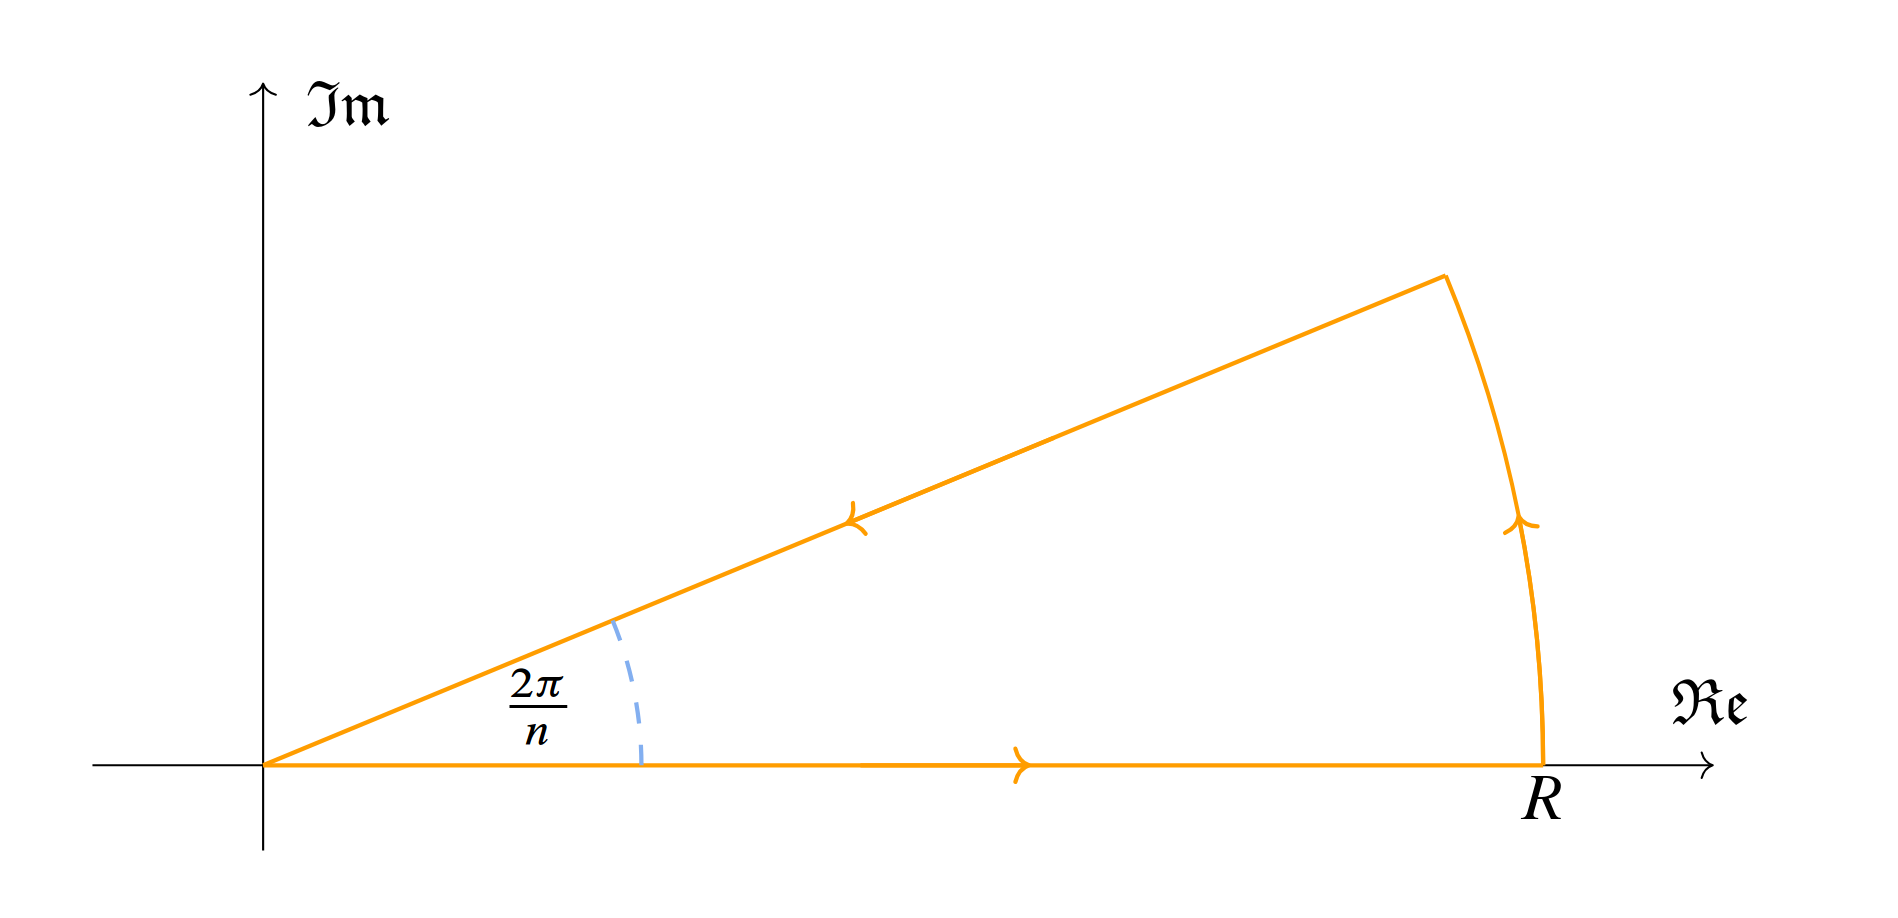
\includegraphics[scale=0.20]{data/complex_analysis/hw5path}
  \end{figure}
  \noindent and conclude by taking $R \to \infty$ that
  \[
    \int_{0}^{\infty} \frac{1}{1 + x^n} \dx =
    \frac{\pi / n}{\sin(\pi / n)}.
  \]
  Notice that we can easily calculate the integral for the case $n = 2$.
  This is one way to find the integral in the general case.
\end{exercise}
\begin{solution}
  
\end{solution}

\subsection{Functions on the circle}
\begin{exercise}
  Let $f \colon C_r(z_0) \to \C$ be continuous.
  We saw in the recitations that the function
  \[
    g(z) := \frac{1}{2 \pi i} \oint_{C_r(z_0)} \frac{f(\omega)}{\omega - z}
    \domega
  \]
  is holomorphic on $D_r(z_0)$, and that
  \[
    g'(z) = \frac{1}{2 \pi i} \oint_{C_r(z_0)} \frac{f(\omega)}{(\omega - z)^2}
    \domega.
  \]
  Prove by induction, using the same steps as in the case $n = 1$ that $g$
  is smooth on $D_r(z_0)$, and
  \[
    g^{(n)}(z) = \frac{n!}{2 \pi i}
    \oint_{C_r(z_0)} \frac{f(\omega)}{(\omega - z)^{n+1}} \domega.
  \]
\end{exercise}
\begin{solution}

\end{solution}

\subsection{Cauchy's theorem}

\begin{exercise}
  Let $\Omega \subset \C$ be a region containing $D_{2r}(z_0)$.
  Show that if $f = u + i v$ is holomorphic on $\Omega$, then
  \[
    u(x_0,y_0) =
    \frac{1}{2 \pi}
    \int_{0}^{2 \pi} u(x_0 + r \cos(\theta), y_0 + r \sin(\theta)) \dtheta.
  \]
  The integral on the right hand side of the equation is called the
  \textit{spherical mean} of $u$.
\end{exercise}
\begin{solution}

\end{solution}

\begin{exercise}
  Let $u(x,y)$ be a harmonic function on
  \[
    U := \set{(x,y) \mid x + i y \in D_{2r}(z_0)}.
  \]
  Prove that $u$ is equivalent to its spherical mean with radius $r$.
  You may find showing that the harmonic conjugate equation
  \[
    v(x,y) =
    \int_{y_0}^{y} \diffp{u}{x}(x,s) \ds -
    \int_{x_0}^{x} \diffp{u}{y}(t,y_0) \dt
  \]
  is satisfied for each $z \in D_{2r}(z_0)$.
\end{exercise}
\begin{solution}

\end{solution}

\begin{exercise}
  Show that if $u(x,y)$ is harmonic, then it has smooth partial derivatives.
\end{exercise}
\begin{solution}

\end{solution}

\newpage
\section{Liouville's theorem and Cauchy's formula}
\subsection{Dense image}
\begin{exercise}
  Let $f \colon \C \to \C$ be entire, such that $f(\C)$ is not dense in $\C$.
  Show that $f$ is constant.
\end{exercise}
\begin{solution}
  Since $f(\C)$ is not dense in $\C$ there exists $\lambda \in \C$ and
  $\epsilon > 0$ such that for all $z \in \C$ we have
  \[
    \abs{f(z) - \lambda} > \epsilon.
  \]
  Define the function
  \[
    g(z) := \frac{1}{f(z) - \lambda}.
  \]
  Since $\abs{f(z) - \lambda} > \epsilon$ we get that $g(z)$ is well
  defined for all $z \in \C$, and as a composition of the entire functions
  $1/z$ and $f(z) - \lambda$ it is also entire.
  We also get that
  \[
    \abs{f(z) - \lambda} > \epsilon
    \implies
    \abs{g(z)} = \abs{\frac{1}{f(z) - \lambda}} \le \frac{1}{\epsilon}
  \]
  so $g$ is bounded.
  Since $g$ is entire and bounded, by Liouville's theorem it is constant.
  We then get that for some constant $C \in \C$,
  \[
    C = \frac{1}{f(z) - \lambda}
    \implies
    f(z) = \frac{1}{C} + \lambda
  \]
  which shows that $f$ is constant and completes the proof.
\end{solution}

\subsection{L'H\^opital's rule and its application}
\begin{exercise} \phantom{}
\begin{enumerate}
  \item[(1)] Let $f(z)$, $g(z)$ be holomorphic functions in a neighbourhood
    of a point $z_0 \in \C$, and let $f(z_0) = g(z_0) = 0$.
    Show that if the limit
    \[
      \lim_{z \to z_0} \frac{f'(z)}{g'(z)}
    \]
    exists then it is equal to
    $\lim_{z \to z_0} \frac{f(z)}{g(z)}$.
  \item[(2)] Let $f \colon \C \to \C$ be entire such that
    for all $z \in \C$
    \[
      \abs{f(z)} \geq \abs{e^z - 1}.
    \]
    Show that $f(z) = C (e^z - 1)$ for some constant $C$.
\end{enumerate}
\end{exercise}
\begin{solution} \phantom{}
\begin{enumerate}
  \item[(1)] Since $f$, $g$ are both holomorphic in a neighbourhood of
    $z_0 \in \C$ and $f(z_0) = g(z_0) = 0$ we can expand both functions
    as series around $z_0$ with some radius of convergence $r > 0$
    \begin{align*}
      f(z) &=
      \sum_{n=n_1}^\infty a_n \cdot (z - z_0)^n =
      (z - z_0)^{n_1} \cdot \sum_{k=0}^{\infty} a_{n_1+k} (z - z_0)^k
      \quad n_1 > 0 \quad a_{n_1} \neq 0 \\
      g(z) &=
      \sum_{n=n_2}^\infty b_n \cdot (z - z_0)^n =
      (z - z_0)^{n_2} \cdot \sum_{k=0}^{\infty} b_{n_2+k} (z - z_0)^k
      \quad n_2 > 0 \quad b_{n_2} \neq 0.
    \end{align*}
    From this it follows that
    \begin{enumerate}

      \item[(1)] If $n_1 = n_2$ then
        $\lim_{z \to z_0} \frac{f(z)}{g(z)} = \frac{a_{n_1}}{b_{n_2}}$. 
      \item[(2)] If $n_1 > n_2$ then
        $\lim_{z \to z_0} \frac{f(z)}{g(z)} = 0$. 
      \item[(3)] If $n_1 < n_2$ then
        $\lim_{z \to z_0} \abs{\frac{f(z)}{g(z)}} = \infty$.
    \end{enumerate}
    In case $(3)$ we take the absolute value because
    $z_n \taking{n \to \infty} \infty$ means
    $\abs{z_n} \taking{n \to \infty} \infty$ by definition.
    Notice that we also have that
    \begin{align*}
      f'(z) &= \sum_{n=n_1}^\infty na_n\cdot (z-z_0)^{n-1}
        = (z - z_0)^{n_1 - 1} \cdot 
        \del{n_1 a_{n_1} + (n_1 + 1) a_{n_1 + 1} (z - z_0) + \dots} \\
      g'(z) &= \sum_{n=n_2}^\infty na_n\cdot (z-z_0)^{n-1}
        = (z - z_0)^{n_2 - 1} \cdot 
        \del{n_2 a_{n_2} + (n_2 + 1) a_{n_2 + 1} (z - z_0) + \dots}.
    \end{align*}
    Applying the same logic gives that in all $3$ cases
    \[
      \lim_{z \to z_0} \frac{f'(z)}{g'(z)} =
      \lim_{z \to z_0} \frac{f(z)}{g(z)}
    \]
    which completes the proof.
  \item[(2)] Define the function
    \[
      g(z) := \frac{f(z)}{e^z - 1}.
    \]
    We see that the denominator vanishes at $z_k = 2 \pi i k$ for $k \in \Z$.
    Consider the limit
    \[
      \lim_{z \to 2 \pi i k} \frac{f'(z)}{[e^z - 1]'} =
      \lim_{z \to 2 \pi i k} \frac{f'(z)}{e^z} =
      \lim_{z \to 2 \pi i k} f'(z) = f'(2 \pi i k).
    \]
    Since this limit exists from $(1)$ it follows that
    \[
      \lim_{z \to 2 \pi i k} \frac{f(z)}{e^z - 1} = f(2 \pi i k).
    \]
    This means that for each $z_k$ there exists $\epsilon_k$ such that
    $g$ is bounded in $D'_{\epsilon_k}(z_k)$ and since it is holomorphic
    on $\C \setminus \set{z_k}_{k \in \Z}$ by a proposition from class the
    points $z_k$ are removable singularities.
    Denote the function without the singularities $\bar g$.
    Since $\bar g$ is holomorphic it is in particular continuous and thus
    $\abs{\bar g(z)} \geq 1$ for all $z \in \C$.
    Since $\bar g$ is entire and bounded from below,
    from Liouville's theorem it must be constant.
    Since $\bar g$ is an extension of $g$ it follows that
    \[
      f(z) = C (e^z - 1)
    \]
    for some constant $C$ which completes the proof.
\end{enumerate}
\end{solution}

\subsection{Cauchy's integral formula}
\begin{exercise} \phantom{}
\begin{enumerate}
  \item[(1)] Calculate the following integrals
    \[
      \oint_{C_1(0)} \frac{e^{z^2}}{z^3 (z^2 + 4)^2} \dz
      \tand
      \oint_{C_2(3i)} \frac{e^{z^2}}{z^3 (z^2 + 4)^2} \dz.
    \]
  \item[(2)] Let $a \in \R$ such that $\abs{a} \neq 1$.
    Show that
    \[
      \int_{0}^{2 \pi} \frac{1}{1 - 2a \cos(\theta) + a^2} \dtheta =
      \frac{2 \pi}{\abs{a^2 - 1}}.
    \]
\end{enumerate}
\end{exercise}
\begin{solution} \phantom{}
\begin{enumerate}
  \item[(1)] Consider the following function
    \[
      f(z) := \frac{e^{z^2}}{z^3 (z^2 + 4)^2}.
    \]
    Denote $Z = \set{-2i,0,2i}$.
    It is clear that $Z$ has no limit point in $\C$,
    $f$ is holomorphic on $\C \setminus Z$,
    and $f$ has a pole at each point at $Z$ and thus $f$ is meromorphic.
    We can now use the residue formula to obtain that
    \[
      \oint_{C_1(0)} \frac{e^{z^2}}{z^3 (z^2 + 4)^2} \dz =
      2 \pi i \sum_{z \in Z} \Ind_{C_1(0)}(z) \cdot \Res(f;z). 
    \]
    Because of the $z^3$ factor $z = 0$ is a pole of order $3$,
    and because of the factor $z = (z^2 + 4)^2$ the poles $\pm 2$
    are of order $2$.
    Using the proposition from class we see that
    \[
      \Res(f;0) = \frac{1}{2!} \lim_{z \to 0} \diff[2]{}{z}
      \left[z^3 f(z)\right].
    \]
    We see that
    \[
      \diff[2]{}{z} \left[z^3 f(z)\right] =
      \diff[2]{}{z} \left[\frac{e^{z^2}}{(z^2 + 4)^2}\right] =
      \frac{2 \left(2z^{6} + 9z^{4} + 18z^{2} + 8\right)
      e^{z^{2}}}{\left(z^{2} + 4\right)^{4}}.
    \]
    This implies that
    \[
      \Res(f;0) = \frac{1}{2!} \lim_{z \to 0} 
      \frac{2 \left(2z^{6} + 9z^{4} + 18z^{2} + 8\right)
      e^{z^{2}}}{\left(z^{2} + 4\right)^{4}} = \frac{1}{2}.
    \]
    We also have that
    \[
      \Res(f;2i) = \lim_{z \to 2i} \diff{}{z} \left[(z - 2i)^2 f(z)\right].
    \]
    Since
    \[
      \diff{}{z} \left[(z - 2i)^2 f(z)\right] =
      \diff{}{z} \left[\frac{e^{z^2}}{z^3 (z + 2i)^2}\right] =
      \frac{\left(2z^{3} + 4i z^{2} - 5z - 6i\right) e^{z^{2}}}{z^{4} \left(z + 2i \right)^{3}}
    \]
    we get that
    \[
      \Res(f;2i) =
      \lim_{z \to 2i} \diff{}{z} \left[z^2 f(z)\right] =
      \lim_{z \to 2i} 
      \frac{\left(2z^{3} + 4i z^{2} - 5z - 6i\right) e^{z^{2}}}{z^{4} \left(z + 2i \right)^{3}} =
      \frac{3}{64 e^4}
    \]
    Similarly we have that
    \begin{align*}
      \Res(f;-2i) &=
      \lim_{z \to -2i} 
      \diff{}{z} \left[(z + 2i)^2 f(z)\right] =
      \lim_{z \to -2i} 
      \diff{}{z} \left[\frac{e^{z^2}}{z^3 (z - 2i)^2}\right] \\ &=
      \lim_{z \to -2i} 
      \frac{\left(2z^{3} - 4i z^{2} - 5z + 6i \right) e^{z^{2}}}{z^{4} \left(z - 2i\right)^{3}} =
      \frac{3}{64 e^4}
    \end{align*}
    This gives us
    \[
      \oint_{C_1(0)} \frac{e^{z^2}}{z^3 (z^2 + 4)^2} \dz =
      2 \pi i \del{\half + 0 + 0} = \pi i
    \]
    and
    \[
      \oint_{C_2(3i)} \frac{e^{z^2}}{z^3 (z^2 + 4)^2} \dz =
      2 \pi i \del{0 + \frac{3}{64 e^4} + 0} = \frac{3 \pi i }{32 e^4}.
    \]
  \item[(2)] As we saw in the recitations
    \[
      \int_{0}^{2 \pi} F(\cos(\theta), \sin(\theta)) \dtheta =
      \oint_{C_1(0)}
      F\del{\frac{z + \frac{1}{z}}{2},\frac{z - \frac{1}{z}}{2i}}
      \frac{\dz}{i z}.
    \]
    Therefore
    \begin{align*}
      I := \int_{0}^{2 \pi} \frac{1}{1 - 2a \cos(\theta) + a^2} \dtheta &=
      \oint_{C_1(0)} \frac{1}{1 - a (z + \frac{1}{z}) + a^2}
      \frac{\dz}{i z} \\ &=
      \oint_{C_1(0)} \frac{1}{z - a (z^2 + 1) + a^2 z}
      \frac{\dz}{i} \\ &=
      \oint_{C_1(0)} \frac{-i}{z - a z^2 - a + a^2 z} \dz \\ &=
      \oint_{C_1(0)} \frac{i}{(z - a)(z - a^{-1}) a} \dz
    \end{align*}
    Assuming $|a| < 1$ we can use Cauchy's integral formula we get that for
    the point $a \in D_1(0)$ by choosing
    \[
      f(z) := \frac{i}{(z - a^{-1}) a}
    \]
    we have that for $|a| < 1$
    \[
      I = 2 \pi i \cdot f(a) \cdot \Ind_{C_1(0)}(a) =
      \frac{- 2 \pi}{a^2 - 1} =
      \frac{2 \pi}{\abs{a^2 - 1}}.
    \]
    Similarly, if $|a| > 1$ then $a^{-1} \in D_1(0)$ and we can do the same
    by choosing
    \[
      f(z) := \frac{i}{(z - a) a}
    \]
    and so for $|a| > 1$
    \[
      I = 2 \pi i \cdot f(a) \cdot \Ind_{C_1(0)}(a) =
      \frac{- 2 \pi}{1 - a^2} =
      \frac{2 \pi}{\abs{a^2 - 1}}.
    \]
    From the above we obtain that for $|a| \neq 1$ we have
    \[
      \int_{0}^{2 \pi} \frac{1}{1 - 2a \cos(\theta) + a^2} \dtheta =
      \frac{2 \pi}{\abs{a^2 - 1}}.
    \]
\end{enumerate}
\end{solution}

\subsection{Generalization of Liouville's theorem}
\begin{exercise}
  Let $f \colon \C \to \C$ be a holomorphic function, and let
  $C > 0$ be a constant such that for some $n \in \N$ we have
  \[
    \abs{f(z)} \le C(1 + \abs{z}^n).
  \]
  Show that $f$ is a polynomial with $\deg(f) \le n$.
\end{exercise}
\begin{solution}
  Since $f$ is entire it is analytic in $\C$.
  This means that it can be written as a series
  \[
    f(z) = \sum_{n=0}^{\infty} \frac{f^{(n)}(0)}{n!} z^n
  \]
  with radius of convergence $\infty$.
  Cauchy's inequalities coupled with the given bound of $f(z)$ gives us
  \[
    \abs{f^{(m)}(z_0)} \le
    \frac{m! \norm{f}_{C_r(z_0)}}{r^m} \le
    \frac{m! C(1 + \del{\abs{z_0} + \abs{r}}^n)}{r^m}
  \]
  for all $r > 0$.
  For $m > n$ by taking $r \to \infty$ we get $f^{(m)}(z_0) = 0$ which
  means that
  \[
    f(z) = \sum_{n=0}^{n} \frac{f^{(n)}(0)}{n!} z^n.
  \]
  This means that $f(z)$ is a polynomial of degree at most $n$ which
  completes the proof.
\end{solution}

\newpage
\section{Cauchy's remainder theorem}

\subsection{Formulas for the remainder}
\begin{exercise}
  \label{ex:remainder-of-f/g}
  Let $f$, $g$ be holomorphic functions in a neighbourhood of $z_0$ such that
  $f(z_0) \neq 0$
  and $z_0$ is a simple zero of $g$.
  Find $\Res(f / g, z_0)$.
\end{exercise}
\begin{solution}
  Let $\Omega$ be a neighbourhood of $z_0$ where $f$, $g$ are holomorphic.
  Since $z_0$ is a simple zero of $g$ there exists a holomorphic
  $h \colon \Omega \to \C$ such that $h(z_0) \neq 0$ and
  \[
    g(z_0) = (z - z_0) h(z) \implies
    g'(z_0) = h(z_0) \neq 0.
  \]
  By a lemma from the notes we have that
  \[
    \Res(f / g, z_0) =
    \lim_{z \to z_0} \frac{f(z)}{g(z)} \overset{\text{L'H\^op}}{=}
    \lim_{z \to z_0} \frac{f(z) + (z - z_0) f(z)}{g'(z)} =
    \frac{f(z_0)}{g(z_0)}
  \]
  where the last inequality follows from the fact $g'$, $f'$ are continuous
  as derivatives of holomorphic functions on $\Omega$.
\end{solution}

\begin{exercise}
  Let $f$ be a meromorphic function in $\C$,
  and suppose that $n \in \Z$ is not a singular point of $f$.
  Find $\Res(\pi \cot (\pi z) f(z), n)$.
\end{exercise}
\begin{solution}
  Recall that
  \[
    \cot(\pi z) =
    \frac{\cos(\pi z)}{\sin(\pi z)}.
  \]
  Since $f$ is meromorphic and $n$ is not a singularity of $f$
  there a exists a neighbourhood of $n$ where $f$ is holomorphic.
  We know that $n$ is a simple zero of $\tan(\pi z)$.
  Thus, since $\cot(z) = z^{-1} \circ \tan(z)$ we get from
  \Cref{ex:remainder-of-f/g} that
  \[
    \Res(\pi \cot(\pi z) f(z),n) = \frac{\pi f(n)}{(\tan(\pi n))'}.
  \]
  Since we have that
  \[
    (\tan(\pi n))' =
    \frac{\pi \cos^{2}(\pi z) + \pi \sin^{2}(\pi z)}{\cos^{2}(\pi z)} =
    \frac{\pi}{\cos^2(\pi z)},
  \]
  we can conclude that
  \[
    \Res(\pi \cot(\pi z) f(z),n) =
    \frac{\pi f(n)}{\frac{\pi}{\cos^2(\pi z)}} =
    f(n)
  \]
  which completes the exercise.
\end{solution}

\subsection{Laurnt series}
\begin{exercise}
  Find the Laurnt series of
  \[
    f(z) := \frac{1}{z^2 - 7z + 12}
  \]
  in the following regions:
  \begin{enumerate}
    \item[(1)] $0 < |z| < 3$;
    \item[(2)] $3 < |z| < 4$;
    \item[(3)] $4 < |z|$.
  \end{enumerate}
\end{exercise}
\begin{solution} \phantom{}
\begin{enumerate}
  \item[(1)] Using partial fraction decomposition we get that
    \[
      f(z) =
      \frac{1}{(z - 3)(z - 4)} =
      \frac{1}{3 - z} - \frac{1}{4 - z} =
      \frac{3}{(1 - \frac{z}{3})} - \frac{4}{(1 - \frac{z}{4})}.
    \]
    In our region we have that $\abs{\frac{z}{4}} < \abs{\frac{z}{4}} < 1$
    which implies that
    \[
      f(z) =
      3 \sum_{n=0}^{\infty} \frac{z^n}{3^n} -
      4 \sum_{n=0}^{\infty} \frac{z^n}{4^n} =
      \sum_{n=0}^{\infty} \del{\frac{3}{3^n} - \frac{4}{4^n}} z^n =
      \sum_{n=0}^{\infty} \del{3^{-(n-1)} - 4^{-(n-1)}} z^n
    \]
    so there are no negative powers in the Laurnt series and we have
    completed this part of the exercise.
  \item[(2)] Recall that we can write the function as
    \[
      f(z) =
      \frac{3}{(1 - \frac{z}{3})} - \frac{4}{(1 - \frac{z}{4})}.
    \]
    In our region we have that $\abs{\frac{z}{4}} < 1$
    which allows us to deal easily with the second summand.
    To deal with the second summand we notice that
    \[
      \frac{3}{\left(1 - \frac{z}{3}\right)} =
      - \frac{1}{z \left(1 - \frac{3}{z}\right)}
    \]
    and since $3 < |z| < 4$ we can expand that we well as such
    \[
      - \frac{1}{z \left(1 - \frac{3}{z}\right)} =
      - \frac{1}{z} \sum_{n=0}^{\infty} 3^n z^{-n}
    \]
    and thus
    \[
      f(z) =
      - \sum_{n=0}^{\infty} 3^{n} z^{-(n+1)}
      - \sum_{n=0}^{\infty} 4^{-(n-1)} z^{n} =
      \sum_{\ninfty}^{\infty} a_n z^n
    \]
    where
    \[
      a_n =
      \begin{cases}
        -4^{-(n-1)}, &n \geq 0 \\
        -3^{n-1}, &n \le -1
      \end{cases}.
    \]
  \item[(3)] As we saw in $(2)$ we can write the function as
    \[
      f(z) =
      \frac{1}{3 - z} - \frac{1}{4 - z} =
      \frac{1}{z \left(1 - \frac{4}{z}\right)} -
      \frac{1}{z \left(1 - \frac{3}{z}\right)}.
    \]
    Since $|z| > 4$ we get that $\abs{\frac{3}{z}} < \abs{\frac{4}{z}} < 1$.
    Thus both summands can be expanded and we get
    \[
      f(z) =
      \frac{1}{z} \sum_{n=0}^{\infty} 4^n z^{-n} -
      \frac{1}{z} \sum_{n=0}^{\infty} 3^n z^{-n} =
      \sum_{n=0}^{\infty} \del{4^n - 3^n} z^{- (n + 1)}
    \]
    so there are no nonnegative powers in the Laurnt series and we have
    completed the last part of the exercise.
\end{enumerate}
\end{solution}

\begin{exercise}
  Find the Laurnt series of
  \[
    f(z) := e^{z + \frac{1}{z}}
  \]
  in the region $|z| > 0$.
\end{exercise}
\begin{solution}
  Using composition of analytic functions we get
  \[
    f(z) =
    \sum_{n=0}^{\infty} \frac{(z + z^{-1})^n}{n!}.
  \]
  We can expand $(z +z^{-1})^n$ as such
  \[
    (z +z^{-1})^n =
    \sum_{k=0}^{n} \binom{n}{k} z^{n - k} \del{z^{-1}}^n =
    \sum_{k=0}^{n} \binom{n}{k} z^{- k}.
  \]
  It follows that
  \[
    f(z) =
    \sum_{n=0}^{\infty} \frac{(z + z^{-1})^n}{n!} =
    \sum_{n=0}^{\infty} \frac{1}{n!} \sum_{k=0}^{n} \binom{n}{k} z^{- k} =
    \sum_{n=0}^{\infty} \sum_{k=0}^{n} \frac{z^{-k}}{(n-k)! k!}.
  \]
  We see that for $k \geq 0$ that
  \[
    a_{-k} =
    \sum_{n=k}^{\infty} \frac{1}{(n - k)! k!} =
    \frac{1}{k!} \sum_{n=k}^{\infty} \frac{1}{(n - k)!} =
    \frac{e}{k!}.
  \]
  This implies that
  \[
    f(z) =
    \sum_{\ninfty}^{\infty} a_n z^n
  \]
  where
  \[
    a_n =
    \begin{cases}
      \frac{e}{(-n)!}, &n \le 0 \\
      0, &n > 0
    \end{cases}.
  \]
\end{solution}

\subsection{Classification of singular points}
\begin{exercise}
  Let $f$ be holomorphic in a set of the form $\set{|z| > R}$ for some
  $R > 0$.
  Define $g(z) := f(1 / z)$.
  Notice that if $f$ is holomorphic, then $0$ is an isolated singularity
  point of $g$.
  In this case we classify the \textit{singularity of $f$ at $\infty$} as the
  singularity of $g$ at $0$.
  \begin{enumerate}
    \item[(1)] Classify the singularity of $f$ at $\infty$ for
      \begin{enumerate}
        \item[(a)] $f(z) := e^z$;
        \item[(b)] $f(z) := \frac{1}{1-z}$;
        \item[(c)] $f(z) := z^n e^{z^{-1}}$.
      \end{enumerate}
    \item[(2)] Show that if $f$ is holomorphic in $\set{|z| > R}$ and
      $\lim_{z \to \infty} f(z) = 0$
      then $f$ has a Laurent series equal to its principle part.
  \end{enumerate}
\end{exercise}
\begin{solution} \phantom{}
\begin{enumerate}
  \item[(1)]
  \begin{enumerate}
    \item[(a)] In this case we have
      \[
        g(z) = f\del{\frac{1}{z}} = e^{z^{-1}}.
      \]
      We have that
      \begin{gather*}
        \lim_{x \to 0^+} e^{z^{-1}} = \infty \\
        \lim_{x \to 0^-} e^{z^{-1}} = 0.
      \end{gather*}
      This implies that $\infty$ is an essential singularity of $f$. 
    \item[(b)] In this case we have
      \[
        g(z) = f\del{\frac{1}{z}} = 1 - z
      \]
      and since we have that
      \[
        \lim_{z \to 0} (1 - z) = 1
      \]
      the point $\infty$ is a removable singularity of $f$.
    \item[(c)] In this case we have
      \[
        g(z) = f\del{\frac{1}{z}} = z^{-n}.
      \]
      If $n = 0$ then $g(z) = 1$ and then $\lim_{z \to 0} g(z) = 1$
      which implies that $\infty$ is a removable singularity of $f$.

      If $n > 0$ then
      \[
        \lim_{z \to 0} \abs{z^{-n}} = \infty
      \]
      which implies that $\infty$ is a pole of $f$.

      Otherwise $n < 0$ so $z^{-n}$ is continuous and thus
      \[
        \lim_{z \to 0} z^{-n} = 0
      \]
      which implies that $\infty$ is a removable singularity of $f$.
  \end{enumerate}
  \item[(2)] Consider the function
    \[
      g(z) = f\del{\frac{1}{z}}.
    \]
    Since the function $\frac{1}{z}$ maps the set $\set{|z| > R}$ to a
    neighbourhood of $0$, it follows that $g$ is holomorphic in a
    neighbourhood of $0$ (excluding $0$).
    Since $\lim_{z \to \infty} f(z) = 0$ it follows that
    $\lim_{z \to 0} g(z) = 0$ which implies that $0$
    is a removable singularity of $g$ which means we can extend $g$ to
    be holomorphic in a neighbourhood of $0$ (including $0$).
    We can then expand $g$ to a Taylor series around $0$ and get
    \[
      g(z) =
      \sum_{n=0}^{\infty} a_n z^n =
      \sum_{n=1}^{\infty} a_n z^n
    \]
    where the last equality follows from $g(0) = 0$.
    We then get
    \[
      f(z) = g\del{\frac{1}{n}} =
      \sum_{n=1}^{\infty} a_n \del{\frac{1}{z}}^n =
      \sum_{n=1}^{\infty} a_n z^{-n} =
      \sum_{\ninfty}^{-1} b_{n} z^{n}
    \]
    where $b_n = a_{-n}$.
    This completes the proof.
\end{enumerate}
\end{solution}

\begin{exercise}
  Suppose $f(z)$ has a simple pole at $z_0$.
  What can you deduce on the singularity type of the function
  $g(z) := e^{f(z)}$ at $z_0$.
\end{exercise}
\begin{solution}
  Since $f$ has a simple pole at $z_0$ there exists $\delta > 0$
  such that $z_0 \in D_{\delta}$ and $f$ is holomorphic on $D'_{\delta}$,
  and there exists a holomorphic function $h \colon D_{\delta} \to \C$
  holomorphic on $D_{\delta}$ such that $f(z) = (z - z_0)^{-1} h(z)$.
  This implies that
  \[
    g(z) =
    e^{h(z)} \cdot e^{\frac{1}{z - z_0}}.
  \]
  We can see that
  \begin{align*}
    \lim_{n \to \infty} \abs{g\del{z_0 + \frac{1}{n}}} &=
    \abs{e^{h(z_0)} \cdot \lim_{n \to \infty} e^{n}} = \infty \\
    \lim_{n \to \infty} \abs{g\del{z_0 - \frac{1}{n}}} &=
    e^{h(z_0)} \cdot \lim_{n \to \infty} e^{-n} = 0.
  \end{align*}
  This implies that $z_0$ is an essential singularity point of $f$.
\end{solution}

\newpage
\section{The residue theorem and the Riemann sphere}

\subsection{The Basel problem}

\begin{exercise} \phantom{}
  \begin{enumerate}
    \item[(1)] Let $a \in \R \setminus \Z$.
      Show that
      \[
        \sum_{n=-\infty}^{\infty} \frac{1}{n^2 + a^2} =
        \frac{\pi \coth(\pi a)}{a}.
      \]
    \item[(2)] Using the sum $\sum_{n \neq 0} \frac{1}{n^2 + a^2}$,
      take $a \to 0^+$ and conclude that
      \[
        \sum_{n=1}^{\infty} \frac{1}{n^2} = \frac{\pi^2}{6}.
      \]
  \end{enumerate}
\end{exercise}
\begin{solution} \phantom{}
\begin{enumerate}
  \item[(1)] Define the function
    \[
      f(z) := \frac{1}{z^2 + a^2}.
    \]
    This function is holomorphic on $\C$ exepct for a finite amount of
    isolated singularity points $A = \set{ia, -ia}$ which are both not in $\Z$.
    We have that exist $k = 2$ and $M = 1$ such that
    \[
      \abs{f(z)} =
      \frac{1}{\abs{z^2 + a^2}} \le
      \frac{1}{\abs{z}^2} =
      \frac{M}{\abs{z}^k}
    \]
    for all $z \in \C$.
    Thus, according to a proposition from the recitations we have that
    \[
      \sum_{n=-\infty}^{\infty} \frac{1}{n^2 + a^2} =
      \sum_{n=-\infty}^{\infty} f(n) =
      - \sum_{z \in A} \Res\del{\pi \cot(\pi z) f(z), z}.
    \]
    According to a proposition from the notes, and since $ia$, $-ia$
    are simple poles we have that
    \begin{small}
    \begin{align*}
      &\Res\del{\pi \cot(\pi z) f(z), ia} =
      \Res\del{\frac{\pi \cot(\pi z)}{z^2 + a^2}, ia} =
      \lim_{z \to ia} \frac{\pi \cot(\pi z)}{z^2 + a^2} (z - ia) =
      \frac{\pi \cot(\pi i a)}{i a + i a} \\
      &\Res\del{\pi \cot(\pi z) f(z), -ia} =
      \Res\del{\frac{\pi \cot(\pi z)}{z^2 + a^2}, -ia} =
      \lim_{z \to -ia} \frac{\pi \cot(\pi z)}{z^2 + a^2} (z + ia) =
      \frac{\pi \cot(- \pi i a)}{- ai - i a}.
    \end{align*}
    Since $\cot$ is an odd function we get that:
    \[
      \sum_{n=-\infty}^{\infty} \frac{1}{n^2 + a^2} =
      - \del{\frac{\pi \cot(\pi i a)}{2 i a} + \frac{\pi \cot(\pi i a)}{2 i a}} =
      - \frac{\pi \cot(\pi i a)}{i a}.
    \]
    Finally, since $\cot(\pi i a) = - i \coth(\pi a)$ we get that
    \[
      \sum_{n=-\infty}^{\infty} \frac{1}{n^2 + a^2} =
      - \frac{\pi \cot(\pi i a)}{i a} =
      \frac{\pi \coth(\pi a)}{a}
    \]
    which completes the first part of the proof.
  \end{small}
  \item[(2)] First we notice that
    \[
      \sum_{n \neq 0} \frac{1}{n^2 + a^2} =
      \sum_{n=-\infty}^{\infty} \frac{1}{n^2 + a^2} - \frac{1}{a^2} =
      \frac{\pi \coth(\pi a)}{a} - \frac{1}{a^2}.
    \]
    It follows that
    \[
      \lim_{a \to 0^+} \sum_{n \neq 0} \frac{1}{n^2 + a^2} =
      \lim_{a \to 0^+} \del{\frac{\pi \coth(\pi a)}{a} - \frac{1}{a^2}} =
      \lim_{a \to 0^+} \del{\frac{\pi \coth(\pi a)}{a} - \frac{1}{a^2}}.
    \]
    Since both $\sinh$ and $\cosh$ are holomorphic on the relevant domain,
    they are analytic and thus,
    \[
      \coth(\pi a) =
      \frac{\cosh(\pi a)}{\sinh(\pi a)} =
      \frac{1 + \frac{(\pi a)^2}{2} + \cdots}
      {\pi a + \frac{(\pi a)^3}{6} + \cdots} = \cdots =
      \frac{1}{\pi a} + \frac{\pi a}{3} + \cdots
    \]
    where the terms after $\frac{\pi a}{3}$ are negligible ($o(a^2)$).
    This gives that
    \[
      \lim_{a \to 0^+} \del{\frac{\pi \coth(\pi a)}{a} - \frac{1}{a^2}} =
      \lim_{a \to 0^+}
      \del{\frac{\pi\del{\frac{1}{\pi a} + \frac{\pi a}{3}}}{a} - \frac{1}{a^2}} =
      \lim_{a \to 0^+}
      \del{\frac{1}{a^2} + \frac{\pi^2}{3} - \frac{1}{a^2}} = \frac{\pi^2}{3}.
    \]
    We also have that:
    \[
      \sum_{n \neq 0} \frac{1}{n^2 + a^2} =
      \sum_{\ninfty}^{-1} \frac{1}{n^2 + a^2} +
      \sum_{n=1}^{\infty} \frac{1}{n^2 + a^2} =
      2 \sum_{n=1}^{\infty} \frac{1}{n^2 + a^2}.
    \]
    So we can conclude that
    \[
      \sum_{n=1}^{\infty} \frac{1}{n^2} =
      \half \lim_{a \to 0^+} \sum_{n \neq 0} \frac{1}{n^2 + a^2} =
      \frac{\pi^2}{6}.
    \]
\end{enumerate}
\end{solution}

\subsection{Corollaries from the Riemann sphere}

\begin{exercise} \phantom{}
  \begin{enumerate}
    \item[(1)] Define the following collections of maps
      \[
        D_r(z) = r z \stand
        T_b(z) = z + b \stand
        R_{\theta}(z) = e^{i \theta} z \stand
        I(z) = \frac{1}{z},
      \]
      where $\theta \in \R$, $b \in \C$, and $0 < r \in \R$.
      Show that $D_r$, $T_b$, $R_{\theta}$ map circles to circles,
      and lines to lines.
    \item[(2)] Show that $I_z$ maps circles and line to
      circles and lines,
      and characterize when the image of a set is a cirlce,
      and when it is a line.
    \item[(3)] A map $f \colon \C_{\infty} \to \C_{\infty}$ is
      call a M\"obius transformation if it is of the form
      \[
        f(z) =
        \begin{cases}
          \frac{a z + b}{c z + d}, &z \neq \infty,-\frac{d}{c} \\
          \infty, &z = -\frac{d}{c} \\
          \frac{a}{c}, &z = \infty
        \end{cases}
      \]
      for $a,b,c,d \in \C$ such that $ad - bc \neq 0$.
      Show that a M\"obius transformation maps circle to circles,
      lines to lines, and characterize when the image is a circle,
      and when it is a line.
    \item[(4)] Find $f(D)$ where
      \[
        f(z) := -i \frac{z + 1}{z - 1}, \quad
        D = \set{\abs{z} < 1}.
      \]
  \end{enumerate}
\end{exercise}
\begin{solution} \phantom{}
\begin{enumerate}
  \item[(1)] 
    First denote the sets
    \begin{align*}
      &L_{v_0} := \set{a v_0 \mid v_0 \in C_1(0) \stand a \in \R} \\
      &C_{r_0} := \set{r_0 v \mid v \in C_1(0) \stand r_0 \in \R}.
    \end{align*}
    Without loss of generality we can show that the maps map these sets
    to a line or a circle.

    We see that
    \[
      D_r(L_{v_0}) = \set{a r v_0 \mid v_0 \in C_1(0) \stand a \in \R \stand r > 0}
    \]
    is a line intersecting the origin in direction $v_0$ and
    \[
      D_r(C_{r_0}) = \set{r r_0 v \mid v \in C_1(0) \stand r_0 \in \R \stand r > 0}
    \]
    is a circle with radius $r r_0$.

    We see that
    \[
      T_b(L_{v_0}) =
      \set{a v_0 + b \mid v_0 \in C_1(0) \stand a \in \R \stand b \in \C}
    \]
    is a line parallel to $v_0$ intersecting the point $b$ and
    \[
      T_b(C_{r_0}) = \set{r_0 v + b \mid v \in C_1(0) \stand r_0 \in \R}
    \]
    is the circle with radius $r_0$ and center $b$.

    We see that
    \[
      R_{\theta}(L_{v_0}) =
      \set{e^{i \theta} a v_0 \mid v_0 \in C_1(0) \stand a \in \R \stand \theta \in \R}
    \]
    is a line intersecting the origin at direction $e^{i \theta} v_0$
    since $e^{i \theta}$ is a unit vector, and it's product with $v_0$
    gives another unit vector on the unit circle. Also
    \[
      R_{\theta}(C_{r_0}) =
      \set{e^{i \theta} r_0 v \mid
      v \in C_1(0) \stand r_0 \in \R \stand \theta \in \R}
    \]
    is a circle since the map $t \colon C_1(0) \to C_1(0)$ given by
    $e^{i \theta} v \mapsto C_1(0)$ is a bijection.
  \item[(2)] Let $\sigma \colon \mathbb S \to \C_{\infty}$ be the stereographic
    projection of the Riemann sphere.
    According to a result from the recitations,
    we have that
    \[
      \frac{1}{z} = \sigma \circ \mathcal I \circ \sigma^{-1}
    \]
    for the function $I(X,Y,Z) = (X,-Y,-Z)$.
    By another result from the recitations,
    we get that if $C \subset \C_{\infty}$ is a circle that contains $0$
    then $\sigma^{-1}$ maps it to a circle in the Riemann sphere that conatins
    $(-1,0,0)$, then $\mathcal I$ maps it to a circle that contains
    $\mathcal N = (1,0,0)$, then $\sigma$ maps it to a line.
    Using the same propositions from the recitations,
    if $C$ does not contain $0$ the map $1/z$ maps it into a line,
    if it is a line that passes through the origin,
    it is mapped to a circle, if it is a line that does not
    pass through the origin, it is mapped to a circle.
    \item[(3)] Since a M\"obius transformation is just the map $1/z$ composed
    with functions from $(1)$ the characterization is the same,
    execpt that instead of asking if the set intersects with the origin,
    we ask if it intersects with $- d / c$.
  \item[(4)] In this case we see that $- d / c = -1$.
    Since the circle $\partial D = C_1(0)$ passes through $- d / c$ it is
    mapped to a line.
    We notice that
    \[
      f(-1) = 0 \tand
      f(i) =
      - i \frac{i + 1}{i - 1} =
      i \frac{(i + 1)^2}{(1 - i)(1 + i)} =
      i \frac{2i}{2} = -1.
    \]
    The only line that passes through these points is $\Im(z) = 0$.
    This implies that $\Im(z) = \partial f(D)$.
    This means that either $f(D) = \mathbb H$ or $f(D) = -\mathbb H$.
    Since $3i = f(1/2) \in \mathbb H$, it follows that $f(D) = \mathbb H$.
\end{enumerate}
\end{solution}

\subsection{Polynomials}

\begin{exercise}
  Let $p(z)$ be a polynomial with $\deg(p) \geq 2$.
  Solve the following subexercises independently.
  \begin{enumerate}
    \item[(1)] Denote $\set{z_k}_k$ the roots of $p$.
      Show that if all the roots are simple, then
      \[
        \sum_{k} \frac{1}{p'(z_k)} = 0.
      \]
    \item[(2)] Show that
      \[
        \lim_{R \to \infty}
        \frac{1}{2 \pi i}
        \oint_{C_R(0)} \frac{p'(z)}{p(z)} \dz = \deg(p).
      \]
    \item[(3)] We denote the upper half-plane as
      $\mathbb H = \set{\Im(z) > 0}$.
      Assume that $p(z)$ has no roots on the real line.
      Show that
      \[
        \int_{\ninfty}^{\infty} \frac{e^{i \omega x}}{p(x)} \dx =
        2 \pi i
        \sum_{\substack{z \in \mathbb H \\ p(z) = 0}}
        \Res\del{\frac{e^{i \omega z}}{p(z)},z}.
      \]
  \end{enumerate}
\end{exercise}
\begin{solution} \phantom{}
\begin{enumerate}
  \item[(1)] Consider the contour integral
    \[
      \oint_{C_R(0)} \frac{1}{p(z)}.
    \]
    Since $\deg p \geq 2$ we have that as $\abs{z} \to \infty$ that
    $\abs{p(z)} \to \infty$.
    Therefore, for a large enough $R > 0$ all the poles of $1/p$,
    which are exactly $\set{z_k}_k$, will be inside $C_R(0)$.

    We can now apply the reside theorem and get
    \[
      \oint_{C_R(0)} \frac{1}{p(z)} =
      2 \pi i \sum_{k} \Res\del{\frac{1}{p(z)}, z_k}.
    \]
    Since each $z_k$ is a simple pole, for $q(z) = (z - z_k)^{-1} p(z)$
    we have $q(z_k) \neq 0$, and thus we get
    \[
      \Res\del{\frac{1}{p(z)}, z_k} =
      \lim_{z \to z_k} (z - z_k) \frac{1}{(z - z_k) q(z)} =
      \frac{1}{q(z_k)}.
    \]
    However we also have
    \[
      p'(z) =
      \left[q(z) (z - z_k)\right]' =
      q(z) + (z - z_k) q'(z) \implies
      q(z_k) = p'(z_k).
    \]
    Thus,
    \[
      \oint_{C_R(0)} \frac{1}{p(z)} =
      2 \pi i \sum_{k} \frac{1}{p'(z_k)}.
    \]
    Note that if we write $p(z) = a^n z^n + \cdots + a_1 z + a_0$ then
    \[
      \lim_{\abs{z} \to \infty} \frac{z^{n}}{p(z)} = a_n
    \]
    which means that for a sufficiently large $R > 0$, the
    function $1 / p$ is bounded by $C / \abs{z}^n$ for some $C > 0$.
    Using the estimation lemma:
    \[
      \abs{\oint_{C_R(0)} \frac{1}{p(z)}} \le
      \frac{2 \pi R \cdot C}{R^{n}} =
      \frac{2 \pi C}{R^{n-1}} \taking{R \to \infty} 0.
    \]
    Where the convergence follows from $n \geq 2$.
    Combining the results we get
    \[
      0 =
      \oint_{C_R(0)} \frac{1}{p(z)} =
      2 \pi i \sum_{k} \Res\del{\frac{1}{p(z)}, z_k} \implies
      \sum_{k} \Res\del{\frac{1}{p(z)}, z_k} = 0
    \]
    which completes the proof.
  \item[(2)] Write
    \[
      p(z) = a^n z^n + a_{n-1} z^{n-1} + \cdots + a_1 z + a_0.
    \]
    Now define
    \begin{align*}
      f(z) &= a^n z^n \\
      g(z) &= a_{n-1} z^{n-1} + \cdots + a_1 z + a_0.
    \end{align*}
    For some sufficiently large $R' > 0$ we have that $\abs{f(z)} > \abs{g(z)}$.
    Since $f$, $g$ are both polynomials, they are entire, and thus we can
    apply Rouche's theorem to obtain that $f$ and $f + g = p$ have the
    same amount of zeros in $D_{R}(0)$ for $R > R'$.

    Since $p(z)$ is a polynomial it is holomorphic, and thus it has no
    poles. Thus, according the the argument principle, for $R > R'$
    \[
        \frac{1}{2 \pi i}
        \oint_{C_R(0)} \frac{p'(z)}{p(z)} \dz =
        \frac{1}{2 \pi i}
        \oint_{C_R(0)} \frac{n a_n z^{n-1}}{a_n z^{n}} \dz =
        \frac{n}{2 \pi i}
        \oint_{C_R(0)} \frac{1}{z} \dz.
    \]
    Using the residue theorem we get
    \[
      \oint_{C_R(0)} \frac{1}{z} \dz =
      2 \pi i \cdot \Res\del{z^{-1}, 0} =
      2 \pi i \cdot \lim_{z \to 0} (z - 0) z^{-1} = 2 \pi i.
    \]
    Combining this with the previous result we get
    \[
        \lim_{R \to \infty}
        \frac{1}{2 \pi i}
        \oint_{C_R(0)} \frac{p'(z)}{p(z)} \dz =
        \lim_{R \to \infty}
        \del{\frac{n}{2 \pi i} \cdot 2 \pi i} = \deg(p)
    \]
    where the first equality follows from the fact that the function inside
    the limit on the LHS is equal to the function inside the limit on the RHS
    for a sufficiently large $R$, and the second equality follows from the
    fact that $n = \deg(p)$.
  \item[(3)] First we define a closed contour $C_R$ consisting of the the real
    axis interval $[-R,R]$ and a positively oriented semicircle $\Gamma_R$
    with radius $R$ centered at the origin.
    We also may assume $\omega > 0$ since otherwise we could repeat the same
    argument for the negatively oriented version of the contour.

    Since $p(z)$ has no roots on the real axis, the reside theorem gives
    \[
      \lim_{R \to \infty} \oint_{C_R} \frac{e^{i \omega x}}{p(x)} =
      2 \pi i
      \sum_{\substack{z \in \mathbb H \\ p(z) = 0}}
      \Res\del{\frac{e^{i \omega z}}{p(z)},z}.
    \]
    We can also see that
    \[
      \oint_{C_R} \frac{e^{i \omega x}}{p(x)} =
      \int_{-R}^{R} \frac{e^{i \omega x}}{p(x)} \dx +
      \oint_{\Gamma_R} \frac{e^{i \omega x}}{p(x)}.
    \]
    Given this we would like to show that the second integral vanishes.
    We can parameterize $\Gamma_R$ by setting $z = R e^{i \theta}$ for
    $\theta \in [0,\pi]$.
    We then have
    \[
      \oint_{\Gamma_R} \frac{e^{i \omega z}}{p(z)} \dz =
      \int_{0}^{\pi}
      \frac{e^{i \omega R e^{i \theta}}}{p(z)} R i e^{i \theta} \dtheta =
      \int_{0}^{\pi}
      \frac{e^{i \omega R \del{\cos \theta + i \sin\theta}}}{p(z)}
      R i e^{i \theta} \dtheta.
    \]
    We then have
    \[
      \int_{0}^{\pi}
      \frac{e^{i \omega R \del{\cos \theta + i \sin\theta}}}{p(z)}
      R i e^{i \theta} \dtheta =
      \int_{0}^{\pi}
      \frac{e^{i \omega R \cos \theta} e^{- \omega R \sin \theta}}
      {p(z)}R i e^{i \theta} \dtheta.
    \]
    Since $\abs{e^{i \omega R \cos \theta}} = 1$ and
    $\abs{i e^{i \theta}} = 1$ we get
    \[
      \abs{\int_{0}^{\pi}
      \frac{e^{i \omega R \cos \theta} e^{- \omega R \sin \theta}}
      {p(z)}R i e^{i \theta} \dtheta} \le
      \int_{0}^{\pi}
      \abs{\frac{e^{i \omega R \cos \theta} e^{- \omega R \sin \theta}}
      {p(z)}R i e^{i \theta}} \dtheta \le
      R \int_{0}^{\pi}
      \frac{e^{- \omega R \sin \theta}}
      {\abs{p(z)}} \dtheta.
    \]
    For $z$ in our semicircle we have that for sufficiently large $R$ that
    for some $c > 0$
    \[
      \abs{p(z)} \geq c R^n \implies
      \frac{1}{\abs{p(z)}} \le \frac{1}{c R^n}.
    \]
    Using this we get
    \[
      R \int_{0}^{\pi}
      \frac{e^{- \omega R \sin \theta}}
      {\abs{p(z)}} \dtheta \le
      \frac{1}{c R^{n-1}}
      \int_{0}^{\pi} e^{- \omega R \sin \theta} \dtheta.
    \]
    Since $\sin$ satisfies the identity $\sin(\theta) = \sin(\pi - \theta)$,
    we can use Jorndan's inqueality (for $\theta \in [0,\pi/2]$ we have
    $\sin \theta \geq \frac{2}{\pi} \theta$) to obtain:
    \[
      \frac{1}{c R^{n-1}}
      \int_{0}^{\pi} e^{- \omega R \sin \theta} \dtheta =
      \frac{2}{c R^{n-1}}
      \int_{0}^{\pi / 2} e^{- \omega R \sin \theta} \dtheta \le
      \frac{2}{c R^{n-1}}
      \int_{0}^{\pi / 2} e^{- \omega R \frac{2}{\pi} \theta} \dtheta.
    \]
    We can now use the substitution $u = \omega R \cdot \frac{2}{\pi} \theta$,
    which implies $\theta = \frac{\pi}{2 \omega R} u$ and
    $\dtheta = \frac{\pi}{2 \omega R} \du$ to compute the integral and get
    \[
      \int_{0}^{\pi / 2} e^{- \omega R \frac{2}{\pi} \theta} \dtheta =
      \frac{\pi}{2 \omega R} 
      \int_{0}^{\omega R} e^{-u} \du =
      \frac{\pi}{2 \omega R} \del{1 - e^{- \omega R}} \le
      \frac{\pi}{2 \omega R}.
    \]
    Combining this with the previous results we can finally write
    \[
      \oint_{\Gamma_R} \frac{e^{i \omega z}}{p(z)} \dz \le
      \frac{2}{c R^{n-1}} \cdot \frac{\pi}{2 \omega R} =
      \frac{\pi}{c \omega R^{n}} \taking{R \to \infty} 0.
    \]
    This shows that
    \[
      \lim_{R \to \infty} \oint_{C_R} \frac{e^{i \omega x}}{p(x)} =
      \int_{\ninfty}^{\infty} \frac{e^{i \omega x}}{p(x)} \dx =
      2 \pi i
      \sum_{\substack{z \in \mathbb H \\ p(z) = 0}}
      \Res\del{\frac{e^{i \omega z}}{p(z)},z}
    \]
    which completes the proof.
\end{enumerate}
\end{solution}

\newpage
\section{The complex logarithm and conformal maps}

\subsection{Roots of order \texorpdfstring{$k$}{k}}
\begin{exercise} \phantom{}
  \begin{enumerate}
    \item[(1)] Let $\Omega \subset \C$ be an open set,
      and let $f \colon \Omega \to \C$ be holomorphic.
      Show that if $z_0 \in \Omega$ is a zero of order $k$ of $f(z)$,
      then there exists a neighbourhood $U$ of $z_0$ in which
      \[
        f(z_0) = \del{z g(z)}^k
      \]
      where $g$ is a holomorphic on $U$ and does not vanish on $U$.
    \item[(2)] Use the open mapping theorem on $z g(z)$, and conclude that
      there exists $r > 0$ so that for all $w \in D'_r(0)$, there exist
      exactly $k$ solutions to the equation $f(z) = w$.
  \end{enumerate}
\end{exercise}
\begin{solution} \phantom{}
\begin{enumerate}
  \item[(1)] Without loss of generality assume that $z_0 = 0$.
    Since $0$ is a zero of $f$ of order $k$ there exists a holomorphic
    function $h(z)$ such that $h(0) \neq 0$ and
    \[
      f(z) = z^k h(z)
    \]
    in a neighbourhood $D_r(0)$ of $0$ for some $r > 0$.
    Since $h$ is holomorphic, it is clear it does not vanish on that
    neighbourhood.
    Since $D_r(0)$ is a region,
    by a theorem from class with $g(z) = f (z)$
    we know that there exists a holomorphic function
    $t \colon D_r(0) \to \C$ such that
    \[
      h(z) = e^{t(z)}.
    \]
    Define the function $g \colon D_r(0) \to \C$ by
    \[
      g(z) := e^{\frac{t(z)}{k}}.
    \]
    Since $g$ is holomorphic, since it does not vanish on $D_r(0)$,
    and since we also have that
    \[
      \del{z g(z)}^k =
      z^k \cdot \del{e^{\frac{t(z)}{k}}}^k =
      z^k \cdot e^{t(z)} =
      z^k \cdot h(z) = f(z)
    \]
    for $z \in D_r(0)$, the proof of the first part of the exercise is done.
  \item[(2)] We can see that $z g(z)$ is not constant since
    $g(z) \neq z^{-1}$, thus $z g(z)$ is an open map.
    We redenote
    \[
      h(z) = z g(z).
    \]
    We have that $h(0) = 0$ and thus $0 \in h(\Omega)$.
    Let $r$ be the radius from part $(1)$ of the exercise
    so that $g(z)$ is defined on $D_r(0)$.
    Since $h$ is an open map we get that $h(D_r(0))$ is an open subset of
    $\C$ which contains $0$.
    Let $1 > r' > 0$ be such that
    \[
      D_{r'}(0) \subset h\del{D_{r}(0)}.
    \]
    Let $w \in D'_{r'}(0)$.
    Since $1 > r'$ the size of the roots must be smaller or equal to the size
    oft the $k$ roots $\sqrt[k] w$ which implies that they must be
    contained inside the punctured disc $ D'_{r'}(0)$.
    We can now solve the equation
    \[
      \del{h(z)}^k = w
    \]
    and see that its solutions are the preimages of the roots $\sqrt[k] w$
    under $h$.
    We also have that
    \[
      h'(0) = g(0) \neq 0
    \]
    so according to the inverse mapping theorem the map $h$ is injective
    at a neighbourood of zero.
    This implies that each root has a unique preimage, so the equation
    \[
      f(z) = \del{h(z)^k} = w
    \]
    has exactly $k$ solutions which completes the proof of the second
    part of the exercise.
\end{enumerate}
\end{solution}

\subsection{Complex powers}
\begin{exercise}
  Recall that if $f$ is analytic on a region $\Omega \subset \C$,
  and $\gamma \colon [a,b] \to \Omega$ is a piecewise-smooth closed path then,
  \[
    \frac{1}{2 \pi i} \oint_{\gamma} \frac{f'(z)}{f(z)} \dz =
    \pm \frac{1}{2 \pi i} \oint_{f \circ \gamma} \frac{1}{z} \dz.
  \]
  \begin{enumerate}
    \item[(1)] Let $0 \neq \alpha \in \C$.
      Show explicitly by definition that
      $\del{z^{\alpha}}' = \alpha z^{\alpha - 1}$ for any adequate region.
    \item[(2)] Let $0 \neq \alpha \in \C$, and suppose that $\Omega \subset \C$
      is an open set that contains the origin.
      Show that if $f \colon \Omega \setminus \set{0} \to \C$ is
      holomorphic and satisfies
      \[
        z f'(z) = \alpha f(z)
      \]
      for all $z \in \Omega \setminus \set{0}$ then $\alpha$ is an integer.
  \end{enumerate}
  Notice that the function $z^{\alpha}$ satisfies
  $z \del{z^{\alpha}}' = \alpha z^{\alpha}$.
  The corollary is that in any open set that contains a deleted neighbourhood
  of the origin, we can't define an analytic branch for $z^{\alpha}$,
  except for the case $\alpha \in \Z$.
\end{exercise}
\begin{solution} \phantom{}
\begin{enumerate}
  \item[(1)] Recall that an adequate region implies that $0 \notin \Omega$
    and $1 \in \Omega$ and that it is simply connected.
    Using the definition of the complex power we get that
    \[
      z^{\alpha} := e^{\alpha \log_{\Omega} z}
    \]
    for each $z \in \Omega$.
    We can now use the chain rule to differentiate this function
    \[
      \diff{z^{\alpha}}{z} =
      \diff{e^{\alpha \log_{\Omega} z}}{z} =
      e^{\alpha \log_{\Omega} z} \cdot \frac{\alpha}{z} =
      \alpha z^{\alpha - 1}
    \]
    which completes the proof.
  \item[(2)] Given the identity $z f'(z) = \alpha f(z)$ we have that
    \[
      \frac{f'(z)}{f(z)} = \frac{\alpha}{z}.
    \]
    We can now take the integral of both sides over a closed path
    that encloses the origin and get
    \[
      \frac{1}{2 \pi i} \oint_{\gamma} \frac{f'(z)}{f(z)} \dz =
      \frac{1}{2 \pi i} \oint_{\gamma} \frac{\alpha}{z} \dz.
    \]
    Using the given integral formula the left hand side is equal to
    \[
      \pm \frac{1}{2 \pi i} \oint_{f \circ \gamma} \frac{1}{z} \dz
    \]
    which is plus or minus the index of $f \circ \gamma$ around the origin,
    which implies this must be an integer.
    We can now proceed to calculate the right side
    using Cauchy's formula in a convex set (the set $\Omega$ is not
    necessarily convex, but since it is open we can work in a convex
    neighbourhood like a disc around the origin) with the function
    $f(z) = 1$ and get
    \[
      \frac{1}{2 \pi i} \oint_{\gamma} \frac{\alpha}{z} \dz =
      \frac{\alpha}{2 \pi i} \oint_{\gamma} \frac{1}{z} \dz =
      \alpha \cdot \Ind_{\gamma}(0) \cdot f(0) = \alpha.
    \]
    Since the lef side of the equality must be an integer,
    and the right side is equal $\alpha$, we must have that
    $\alpha$ is an integer which completes the proof.
\end{enumerate}
\end{solution}

\subsection{Applications of Schwartz's lemma}
\begin{exercise}
  Let $f \colon \mathbb D \to \mathbb D$ be holomorphic.
  Show that
  \[
    \abs{\frac{f(z) - f(w)}{1 - \overline{f(w)} f(z)}} \le
    \abs{\frac{z - w}{1 - \overline w z}} % This is smaller than 1 sometimes
  \]
  for all $z,w \in \mathbb D$.
\end{exercise}
\begin{solution}
  Let $h_{w}(z)$ be the function
  \[
    h_w(z) := \psi_{f(w)} \circ f \circ \psi_{w}(z)
  \]
  where $\psi_{w}$ is the automorphism of the disc
  \[
    \psi_{w}(z) = \frac{z - w}{z \overline w - 1}.
  \]
  We see that
  \[
    h_w(0) =
    \psi_{f(w)} \circ f \circ \psi_{w}(0) =
    \psi_{f(w)} \circ f(w) = 0.
  \]
  Thus from Schwartz's lemma we get that
  \[
    \abs{h_w(z)} \le \abs{z}
  \]
  for all $z \in \mathbb D$.
  Explicitly, since $\psi_w(z)$ is the inverse of itself we have that
  \[
    h_w \circ \psi_w(z) =
    \psi_{f(w)} \circ f(z) =
    \frac{f(z) - f(w)}{\overline{f(w)} f(z) - 1}.
  \]
  However, from Schwartz's lemma we have
  \[
    \abs{h_w \circ \psi_w(z)} \le
    \abs{\psi_w(z)} =
    \abs{\frac{z - w}{\overline w z - 1}} =
    \abs{\frac{z - w}{1 - \overline w z}}.
  \]
  Combining the results we have
  \[
    \abs{\frac{f(z) - f(w)}{\overline{f(w)} f(z) - 1}} =
    \abs{\frac{f(z) - f(w)}{1 - \overline{f(w)} f(z)}} \le
    \abs{\frac{z - w}{1 - \overline w z}}
  \]
  which completes the proof.
\end{solution}


\end{document}
